% Orbital Mechanics for Propulsion Engineers -- the astrodynamics behind mission_analysis
% Build (from this directory):  latexmk -pdf orbital_mechanics_tutorial.tex
% Numbers: tutorial_numbers.tex (calc/make_tutorial_numbers.py); figures: figs/ (calc/make_tutorial_figures.py)
\documentclass[11pt,letterpaper,oneside]{report}
\usepackage[margin=1in]{geometry}
\usepackage[T1]{fontenc}
\usepackage[utf8]{inputenc}
\usepackage{lmodern}
\usepackage{microtype}
\usepackage{amsmath,amssymb,mathtools,bm}
\usepackage{siunitx}
\usepackage{booktabs}
\usepackage{graphicx}
\usepackage{xcolor}
\usepackage{enumitem}
\usepackage[font=small,labelfont=bf]{caption}
\usepackage{subcaption}
\usepackage{titlesec}
\usepackage{fancyhdr}
\usepackage[most]{tcolorbox}
\usepackage{tikz}
\usetikzlibrary{calc,arrows.meta,decorations.markings,angles,quotes,positioning}
\usepackage{listings}
\usepackage{hyperref}
\usepackage[nameinlink,capitalise]{cleveref}

\graphicspath{{figs/}}
% AUTO-GENERATED by calc/make_tutorial_numbers.py -- do not edit by hand
\newcommand{\muEarth}{398600.4}
\newcommand{\REarth}{6378.1}
\newcommand{\muSun}{1.3271e+11}
\newcommand{\muMoon}{4902.8}
\newcommand{\muMars}{42828.4}
\newcommand{\muJupiter}{1.2671e+08}
\newcommand{\ISSvc}{7.657}
\newcommand{\ISSperiodmin}{93.0}
\newcommand{\ISSvesc}{10.829}
\newcommand{\ISSenergy}{-29.32}
\newcommand{\GEOa}{42164}
\newcommand{\GEOalt}{35786}
\newcommand{\GEOvc}{3.075}
\newcommand{\GTOa}{24421}
\newcommand{\GTOe}{0.7265}
\newcommand{\GTOvp}{10.151}
\newcommand{\GTOva}{1.608}
\newcommand{\GTOperiodh}{10.55}
\newcommand{\GTOenergy}{-8.161}
\newcommand{\GTOh}{67793}
\newcommand{\GTOp}{11530}
\newcommand{\GTOEninety}{43.40}
\newcommand{\GTOMninety}{14.80}
\newcommand{\GTOtninetymin}{26.0}
\newcommand{\GTOhalfperiodmin}{316.5}
\newcommand{\HohLEOGEOdvone}{2.426}
\newcommand{\HohLEOGEOdvtwo}{1.467}
\newcommand{\HohLEOGEOtot}{3.893}
\newcommand{\HohLEOGEOtofh}{5.28}
\newcommand{\HohLEOGEOvtp}{10.151}
\newcommand{\HohLEOGEOvta}{1.608}
\newcommand{\HohLEOGEOvcone}{7.726}
\newcommand{\HohLEOGEOvctwo}{3.075}
\newcommand{\HohPCdvone}{2.449}
\newcommand{\HohPCdvtwo}{1.782}
\newcommand{\HohPCtot}{4.231}
\newcommand{\HohPCdione}{2.20}
\newcommand{\HohPCditwo}{26.30}
\newcommand{\PCatLEO}{3.803}
\newcommand{\PCatGEO}{1.514}
\newcommand{\HohPeakRatio}{15.57}
\newcommand{\HohPeakValue}{0.5363}
\newcommand{\HohEscapeLimit}{0.4142}
\newcommand{\BiEllTot}{3.994}
\newcommand{\BiEllHoh}{4.046}
\newcommand{\BiEllTOFd}{13.4}
\newcommand{\BiEllHohTOFh}{18.3}
\newcommand{\SynEM}{779.9}
\newcommand{\PhaseEM}{44.3}
\newcommand{\SOIEarth}{929}
\newcommand{\SOIMoon}{66}
\newcommand{\SOIMars}{577}
\newcommand{\SOIJupiter}{48210}
\newcommand{\SOIVenus}{616}
\newcommand{\SOISaturn}{54551}
\newcommand{\SOIEarthAU}{0.0062}
\newcommand{\EMvtp}{32.729}
\newcommand{\EMvta}{21.480}
\newcommand{\EMvEarth}{29.785}
\newcommand{\EMvMars}{24.129}
\newcommand{\EMvinfdep}{2.945}
\newcommand{\EMvinfarr}{2.649}
\newcommand{\EMCthree}{8.67}
\newcommand{\EMtofd}{258.9}
\newcommand{\EMdvdep}{3.590}
\newcommand{\EMvhyp}{11.316}
\newcommand{\EMvpark}{7.726}
\newcommand{\EMehyp}{1.145}
\newcommand{\EMturnhalf}{29.2}
\newcommand{\EMcapcirc}{2.080}
\newcommand{\EMcapell}{0.884}
\newcommand{\EMcapvhyp}{5.439}
\newcommand{\EMcapvc}{3.359}
\newcommand{\EMcapvpell}{4.555}
\newcommand{\EMcapOptRp}{12207}
\newcommand{\EMcapOptAlt}{8811}
\newcommand{\Obvinf}{3.0}
\newcommand{\Obdv}{3.604}
\newcommand{\Obesc}{3.200}
\newcommand{\ObvescLEO}{10.926}
\newcommand{\PlVenusvinfdep}{2.50}
\newcommand{\PlVenusCthree}{6.2}
\newcommand{\PlVenusdvdep}{3.48}
\newcommand{\PlVenusvinfarr}{2.71}
\newcommand{\PlVenustofd}{146}
\newcommand{\PlVenusphase}{-54.0}
\newcommand{\PlVenussyn}{1.60}
\newcommand{\PlMarsvinfdep}{2.94}
\newcommand{\PlMarsCthree}{8.7}
\newcommand{\PlMarsdvdep}{3.59}
\newcommand{\PlMarsvinfarr}{2.65}
\newcommand{\PlMarstofd}{259}
\newcommand{\PlMarsphase}{44.3}
\newcommand{\PlMarssyn}{2.14}
\newcommand{\PlJupitervinfdep}{8.79}
\newcommand{\PlJupiterCthree}{77.3}
\newcommand{\PlJupiterdvdep}{6.30}
\newcommand{\PlJupitervinfarr}{5.64}
\newcommand{\PlJupitertofd}{998}
\newcommand{\PlJupiterphase}{97.2}
\newcommand{\PlJupitersyn}{1.09}
\newcommand{\PlSaturnvinfdep}{10.29}
\newcommand{\PlSaturnCthree}{105.9}
\newcommand{\PlSaturndvdep}{7.28}
\newcommand{\PlSaturnvinfarr}{5.44}
\newcommand{\PlSaturntofd}{2208}
\newcommand{\PlSaturnphase}{106.1}
\newcommand{\PlSaturnsyn}{1.04}
\newcommand{\GAJupiterturn}{149.5}
\newcommand{\GAJupiterdv}{15.43}
\newcommand{\GAVenusturn}{52.7}
\newcommand{\GAVenusdv}{7.11}
\newcommand{\GAEarthturn}{57.7}
\newcommand{\GAEarthdv}{7.72}
\newcommand{\VgCthree}{104.7}
\newcommand{\Vgvinfin}{7.898}
\newcommand{\Vgvinfout}{7.775}
\newcommand{\Vgturn}{97.0}
\newcommand{\Vgrp}{692}
\newcommand{\Vghelio}{11.74}
\newcommand{\Vgvin}{9.64}
\newcommand{\Vgvout}{19.65}
\newcommand{\Vgdvpow}{0.047}
\newcommand{\EphLonEarth}{49.2}
\newcommand{\EphLonMars}{105.6}
\newcommand{\EphPhase}{56.4}
\newcommand{\EphrEarth}{0.9900}
\newcommand{\EphrMars}{1.6058}
\newcommand{\EphvEarth}{30.085}
\newcommand{\EphvMars}{22.863}
\newcommand{\EphdistEM}{1.341}
\newcommand{\EphMoonDist}{404165}
\newcommand{\EphMoonSpeed}{0.975}
\newcommand{\EphT}{0.268624}
\newcommand{\EphMarsa}{1.523715}
\newcommand{\EphMarse}{0.093415}
\newcommand{\EphMarsM}{120.82}
\newcommand{\EphMarsnu}{129.46}
\newcommand{\LamCthree}{9.21}
\newcommand{\Lamvinfdep}{3.035}
\newcommand{\Lamvinfarr}{2.574}
\newcommand{\Lamtofd}{311}
\newcommand{\Lamdtheta}{206.2}
\newcommand{\Lama}{1.2693}
\newcommand{\Lamdvdep}{3.614}
\newcommand{\Lamdvcap}{2.044}
\newcommand{\LamrOneAU}{0.9932}
\newcommand{\LamrTwoAU}{1.5197}
\newcommand{\LamvOne}{32.977}
\newcommand{\LamvE}{29.988}
\newcommand{\PkOptDep}{2026-10-30}
\newcommand{\PkOptTOF}{311}
\newcommand{\PkOptCthree}{9.22}
\newcommand{\PkOptvinfarr}{2.572}
\newcommand{\PkOptdv}{5.657}
\newcommand{\PkOptAngle}{206}
\newcommand{\PkMinCthree}{9.14}
\newcommand{\PkMinCthreeDep}{2026-10-30}
\newcommand{\PkMinCthreeTOF}{293}
\newcommand{\PkWinOpen}{2026-09-20}
\newcommand{\PkWinClose}{2026-11-30}
\newcommand{\PkWinDays}{70}
\newcommand{\PkTypeIDep}{2026-11-16}
\newcommand{\PkTypeITOF}{260}
\newcommand{\PkTypeICthree}{12.00}
\newcommand{\PkTypeIvinf}{3.037}
\newcommand{\PkTypeIdv}{6.015}
\newcommand{\MtwCthree}{14.50}
\newcommand{\Mtwvinfarr}{2.552}
\newcommand{\Mtwtof}{203}
\newcommand{\Mtwdtheta}{143.1}
\newcommand{\MtwPath}{470.9}
\newcommand{\MtwEntry}{5.55}
\newcommand{\MoonD}{384400}
\newcommand{\MoonSOI}{66183}
\newcommand{\MoonV}{1.0232}
\newcommand{\MoonSOIfrac}{17}
\newcommand{\LunTLIv}{10.9283}
\newcommand{\LunTLIdv}{3.135}
\newcommand{\Lunvpark}{7.793}
\newcommand{\LunTOFd}{4.98}
\newcommand{\Lunvapo}{0.1866}
\newcommand{\Lunvinf}{0.8366}
\newcommand{\LunLOI}{0.823}
\newcommand{\LunLOIvhyp}{2.457}
\newcommand{\LunLOIvc}{1.634}
\newcommand{\Luntot}{3.959}
\newcommand{\Lunat}{195482}
\newcommand{\LunRlam}{44.1}
\newcommand{\LunRtofgeo}{56.9}
\newcommand{\LunRtofsoi}{15.4}
\newcommand{\LunRtoftot}{72.3}
\newcommand{\LunRvinf}{1.078}
\newcommand{\LunRLOI}{0.886}
\newcommand{\LunRTLI}{3.157}
\newcommand{\LunRrone}{340}
\newcommand{\LunRvone}{0.884}
\newcommand{\LunRphione}{76.2}
\newcommand{\LunRgammaone}{7.78}
\newcommand{\LunRlead}{131.8}
\newcommand{\LunRetwo}{1.380}
\newcommand{\LunRa}{255}
\newcommand{\LunRe}{0.9742}
\newcommand{\LunPlam}{35.9}
\newcommand{\LunPtofgeo}{54.7}
\newcommand{\LunPtofsoi}{15.1}
\newcommand{\LunPtoftot}{69.8}
\newcommand{\LunPvinf}{1.108}
\newcommand{\LunPLOI}{0.899}
\newcommand{\LunPTLI}{3.157}
\newcommand{\LunProne}{333}
\newcommand{\LunPvone}{0.911}
\newcommand{\LunPphione}{76.3}
\newcommand{\LunPgammaone}{6.70}
\newcommand{\LunPlead}{133.8}
\newcommand{\LunPetwo}{1.404}
\newcommand{\LunPa}{255}
\newcommand{\LunPe}{0.9742}
\newcommand{\ApTOF}{67.8}
\newcommand{\ApLOI}{0.919}
\newcommand{\Aplam}{40.1}
\newcommand{\ApTOFtwo}{69.5}
\newcommand{\ApLOItwo}{0.905}
\newcommand{\LchVorb}{7.726}
\newcommand{\LchVsite}{0.409}
\newcommand{\LchIdeal}{7.317}
\newcommand{\LchLow}{8.47}
\newcommand{\LchHigh}{9.37}
\newcommand{\LchOmega}{7.2921e-05}
\newcommand{\LchVeq}{0.465}
\newcommand{\LchISSaz}{45.0}
\newcommand{\LchISSsite}{0.534}
\newcommand{\LchISScredit}{0.283}
\newcommand{\LchISSideal}{7.442}
\newcommand{\LchPolarIdeal}{7.737}
\newcommand{\LchPolarCredit}{-0.011}
\newcommand{\LchKourouCredit}{0.463}
\newcommand{\AcEntry}{5.598}
\newcommand{\AcSaved}{2.080}
\newcommand{\AcRaise}{0.0637}
\newcommand{\AcNet}{2.016}
\newcommand{\AbPasses}{521}
\newcommand{\AbDays}{152}
\newcommand{\AbDrag}{1.192}
\newcommand{\AbCapHigh}{0.853}
\newcommand{\AbRaise}{0.066}
\newcommand{\AbDirect}{2.080}
\newcommand{\AbSaved}{1.161}
\newcommand{\AbFirst}{1.95}
\newcommand{\AbRho}{5.79e-08}
\newcommand{\AbVp}{4.754}
\newcommand{\AbNum}{1.951}
\newcommand{\AbAna}{1.952}
\newcommand{\AbStraight}{1.323}
\newcommand{\AbFactor}{1.475}
\newcommand{\AbH}{10.5}
\newcommand{\AbRddot}{2.9630}
\newcommand{\gzero}{9.80665}
\newcommand{\ZetaThreeTwoZero}{0.837}
\newcommand{\ZetaFourFiveZero}{0.725}
\newcommand{\ZetaNineZeroZero}{0.476}
\newcommand{\ZetaThreeZeroZeroZero}{0.176}
\newcommand{\IspSSTO}{412}
\newcommand{\HWdepart}{2026-10-30}
\newcommand{\HWarrive}{2027-09-06}
\newcommand{\HWlaunchMid}{8.917}
\newcommand{\HWinj}{3.614}
\newcommand{\HWcap}{2.043}
\newcommand{\HWmargin}{0.729}
\newcommand{\HWtotProp}{15.303}
\newcommand{\HWtotAero}{13.225}
\newcommand{\HWpostProp}{6.386}
\newcommand{\HWpostAero}{4.308}
\newcommand{\HWIspPropFive}{939}
\newcommand{\HWIspAeroFive}{634}
\newcommand{\HWIspPropSix}{711}
\newcommand{\HWIspAeroSix}{479}
\newcommand{\HWIspPropSeven}{541}
\newcommand{\HWIspAeroSeven}{365}
\newcommand{\HWminj}{7652}
\newcommand{\HWmpropInj}{5233}
\newcommand{\HWmpropCap}{1157}
\newcommand{\HWmpropMargin}{261}
\newcommand{\HWdvLauncher}{12.531}
\newcommand{\HWmZero}{694}
\newcommand{\HWpf}{1.10}
\newcommand{\HWdvB}{4.822}
\newcommand{\HWdvU}{7.709}
\newcommand{\HWmB}{601}
\newcommand{\HWmU}{85.0}
\newcommand{\HWmZeroeq}{924}
\newcommand{\HWcLow}{2.942}
\newcommand{\HWcUp}{4.413}
\newcommand{\ExMarsVc}{3.315}
\newcommand{\ExMarsTmin}{123.1}
\newcommand{\ExMarsVesc}{4.689}
\newcommand{\ExLunHohdvone}{3.082}
\newcommand{\ExLunHohdvtwo}{0.829}
\newcommand{\ExLunHohtot}{3.911}
\newcommand{\ExLunHohtofd}{4.98}
\newcommand{\ExLunHohvta}{0.190}
\newcommand{\ExLunHohvcTwo}{1.018}
\newcommand{\ExJupvinf}{5.643}
\newcommand{\ExJupCapCirc}{17.586}
\newcommand{\ExJupCapEll}{1.277}
\newcommand{\ExJupVhyp}{59.395}
\newcommand{\ExJupVc}{41.809}
\newcommand{\ExJupOptAlt}{7886}
\newcommand{\ExVenTurn}{84.4}
\newcommand{\ExVenDv}{6.717}
\newcommand{\ExVenE}{1.489}
\newcommand{\ExBaikSite}{0.324}
\newcommand{\ExBaikIdeal}{7.402}
\newcommand{\ExBaikISSideal}{7.438}
\newcommand{\ExBaikISSaz}{63.2}
\newcommand{\ExAbPasses}{1041}
\newcommand{\ExAbDays}{304}
\newcommand{\ExIspReq}{419}
\newcommand{\ExZeta}{0.747}
\newcommand{\ExLunTOF}{54.3}
\newcommand{\ExLunLOI}{1.100}
\newcommand{\ExLunTLI}{3.207}
\newcommand{\ExLunLam}{29.1}
\newcommand{\ExLegCthree}{11.87}
\newcommand{\ExLegvinf}{3.046}
\newcommand{\ExLegAngle}{172}
\newcommand{\ExLegTOF}{260}
\newcommand{\ExVinfFromBurn}{2.577}
\newcommand{\ExCthreeFromBurn}{6.64}


% ---------- Columbia palette (matches the Rocket Module notes)
\definecolor{CUblue}{RGB}{1,33,105}
\definecolor{CUlight}{RGB}{108,172,228}
\definecolor{CUmagenta}{RGB}{212,40,91}
\definecolor{CUteal}{RGB}{37,155,154}
\definecolor{CUpurple}{RGB}{123,42,141}
\definecolor{sfblue}{HTML}{2A78D6}
\definecolor{sforange}{HTML}{EB6834}
\definecolor{sfgray}{HTML}{898781}
\hypersetup{colorlinks,linkcolor=CUblue,citecolor=CUblue,urlcolor=CUteal}

\titleformat{\chapter}[display]{\normalfont\huge\bfseries\color{CUblue}}{\chaptertitlename\ \thechapter}{10pt}{\Huge}
\titleformat{\section}{\normalfont\Large\bfseries\color{CUblue}}{\thesection}{1em}{}
\titleformat{\subsection}{\normalfont\large\bfseries\color{CUblue!80!black}}{\thesubsection}{1em}{}
\titlespacing*{\chapter}{0pt}{-20pt}{30pt}

\pagestyle{fancy}\fancyhf{}
\fancyhead[L]{\small\color{CUblue}Orbital Mechanics for Propulsion Engineers}
\fancyhead[R]{\small\nouppercase{\leftmark}}
\fancyfoot[C]{\thepage}
\renewcommand{\headrulewidth}{0.4pt}

\sisetup{per-mode=symbol,separate-uncertainty=true,range-phrase=--,range-units=single,detect-all}
\DeclareSIUnit{\AU}{AU}\DeclareSIUnit{\year}{yr}\DeclareSIUnit{\days}{d}

% ---------- call-out boxes
\newtcolorbox{keyresult}{enhanced,colback=white,colframe=CUteal,boxrule=0.8pt,left=4pt,right=4pt,top=3pt,bottom=3pt}
\newtcolorbox{worked}[1]{enhanced,colback=CUlight!10,colframe=CUblue,fonttitle=\bfseries,title={Worked example -- #1},left=4pt,right=4pt,top=3pt,bottom=3pt}
\newtcolorbox{codebox}{enhanced,colback=gray!6,colframe=gray!50,boxrule=0.4pt,fontupper=\small,title={Where this lives in \code{mission\_analysis}},fonttitle=\bfseries\small,left=4pt,right=4pt,top=2pt,bottom=2pt}
\newtcolorbox{pitfall}{enhanced,colback=CUmagenta!6,colframe=CUmagenta,boxrule=0.6pt,fontupper=\small,title={Pitfall},fonttitle=\bfseries\small,left=4pt,right=4pt,top=2pt,bottom=2pt}
\newtcolorbox{propulsion}{enhanced,colback=CUpurple!6,colframe=CUpurple,boxrule=0.6pt,fontupper=\small,title={For the propulsion engineer},fonttitle=\bfseries\small,left=4pt,right=4pt,top=2pt,bottom=2pt}

\lstset{language=Python,basicstyle=\ttfamily\footnotesize,columns=fullflexible,keepspaces=true,breaklines=true,
  frame=single,framerule=0.3pt,rulecolor=\color{sfgray},xleftmargin=4pt,xrightmargin=4pt,
  keywordstyle=\color{CUblue},commentstyle=\color{sfgray},stringstyle=\color{CUteal},showstringspaces=false}

% ---------- notation (one meaning per symbol; aligned with the notes' Appendix A)
\newcommand{\dv}{\Delta v}
\newcommand{\vinf}{v_\infty}
\newcommand{\En}{\mathcal E}
\newcommand{\Isp}{{I_{sp}}}
\newcommand{\gz}{g_0}
\newcommand{\dd}{\mathrm{d}}
\newcommand{\code}[1]{\texttt{#1}}
\newcommand{\bv}[1]{\bm{#1}}
\newcommand{\uv}[1]{\hat{\bm{#1}}}

\title{\color{CUblue}\textbf{Orbital Mechanics for Propulsion Engineers}\\[6pt]
\Large The astrodynamics behind \code{mission\_analysis}\\[4pt]
\large a tutorial for engineers who know thermodynamics and dynamics\\ but have not met orbits}
\author{MECE 4305 -- Mechanics \& Thermodynamics of Propulsion, Rocket Module\\Columbia University, Fall 2026}
\date{November 2026}

\begin{document}
\maketitle

\chapter*{How to read this tutorial}
\addcontentsline{toc}{chapter}{How to read this tutorial}

You know Newton's laws, energy and momentum, ODEs and vector calculus, and you know what a
rocket engine does: it produces a velocity increment $\dv$ at a propellant cost set by the rocket
equation. What you may not know is where the $\dv$ numbers in a mission come from. This tutorial
builds that knowledge from the two-body problem up to the point where you can read, trust and
extend every function in the \code{mission\_analysis} package (the \code{sfmission} tool used in
Week~10 and HW~1).

Each chapter follows the same pattern: the physics, derived at the level a mechanical engineer
expects; a \emph{worked example} with numbers computed by the package itself (every number in
this document is generated by \code{calc/make\_tutorial\_numbers.py}, so text and code cannot
drift apart); a \emph{code box} naming the functions that implement the result; a \emph{pitfall}
where experience says people go wrong; and a few exercises, with answers in \cref{app:answers}.

\begin{center}\small
\begin{tabular}{lll}\toprule
Chapter & Question it answers & Module \\\midrule
1 & How does a body move around a central mass? & \code{kepler} \\
2 & How much $\dv$ does it take to change an orbit? & \code{transfers} \\
3 & How do we leave one body for another? & \code{patched\_conics} \\
4 & Where are the planets on a given date? & \code{ephemeris} \\
5 & What transfer connects two positions in a given time? & \code{lambert}, \code{porkchop} \\
6 & Why is the Moon a special case? & \code{lunar} \\
7 & What does it cost to reach orbit? & \code{launch} \\
8 & How does an atmosphere save propellant? & \code{aerobraking} \\
9 & How does $\dv$ become propellant and stages? & \code{staging}, \code{budget} \\
10 & Putting it together: a Mars orbiter & all \\\bottomrule
\end{tabular}
\end{center}

\paragraph{Units and symbols.} Kilometres, seconds and kilograms; angles in radians in formulas
and degrees in text. One meaning per symbol: $\mu$ is \emph{only} the gravitational parameter
$GM$; $\En$ is specific mechanical energy; $\zeta$, $\sigma_i$, $\pi_i$, $R_i$ are the mass
fractions of the lecture notes (\cref{ch:staging}); $\varepsilon$ is reserved for nozzle area
ratio and never appears here. A full table is in \cref{app:symbols}.

\tableofcontents

%==================================================================
\chapter{One body around another: the two-body problem}\label{ch:twobody}
%==================================================================

\section{Setting up the problem}
Two point masses $M$ (planet) and $m$ (spacecraft) attract each other with Newton's force. Writing
the equation of motion of each and subtracting, the \emph{relative} position $\bv r$ of the
spacecraft with respect to the planet obeys
\begin{equation}
  \ddot{\bv r} = -\frac{G(M+m)}{r^3}\,\bv r \;\approx\; -\frac{\mu}{r^3}\,\bv r,\qquad \mu\equiv GM ,
  \label{eq:eom}
\end{equation}
because $m\ll M$. Everything that follows is a consequence of \cref{eq:eom}. Two remarks before
we solve it. First, $\mu$ is what is measured (from spacecraft tracking) and is known to ten
digits, while $G$ and $M$ separately are known to only five; always work with $\mu$. Second, the
``point mass'' assumption is excellent outside the atmosphere for a body that is nearly spherical:
Earth's oblateness ($J_2$) changes orbits slowly, which matters for satellites over years but not
for a transfer that lasts days.

\begin{center}\small
\begin{tabular}{lcc}\toprule
Body & $\mu$ [\si{km^3/s^2}] & mean radius [km] \\\midrule
Sun & $\muSun$ & 695,700 \\
Earth & $\muEarth$ & $\REarth$ \\
Moon & $\muMoon$ & 1,737.4 \\
Mars & $\muMars$ & 3,396.2 \\
Jupiter (system) & $\muJupiter$ & 71,492 \\\bottomrule
\end{tabular}
\end{center}

\section{What is conserved}
\paragraph{Angular momentum.} Cross \cref{eq:eom} with $\bv r$: the right side vanishes, so
$\dd(\bv r\times\dot{\bv r})/\dd t=0$ and
\begin{equation}
  \bv h \equiv \bv r\times\bv v = \text{const}.
\end{equation}
$\bv h$ is the specific angular momentum (per unit mass). Because $\bv r$ is always perpendicular
to the fixed vector $\bv h$, \emph{the motion lies in a plane}. In polar coordinates in that plane
$h = r^2\dot\nu$, which is Kepler's second law (equal areas in equal times) and, as we will see,
the reason a spacecraft lingers at apoapsis and races through periapsis.

\paragraph{Energy.} Dot \cref{eq:eom} with $\bv v$: $\bv v\cdot\dot{\bv v} = -\mu\,\bv r\cdot\bv v/r^3 = -\mu\dot r/r^2 = \dd(\mu/r)/\dd t$, so
\begin{keyresult}
\begin{equation}
  \En \equiv \frac{v^2}{2}-\frac{\mu}{r} = \text{const}.
  \label{eq:energy}
\end{equation}
\end{keyresult}
$\En<0$: the spacecraft cannot reach $r\to\infty$ (bound, elliptical). $\En=0$: it arrives at
infinity with zero speed (parabolic). $\En>0$: it arrives with a residual speed $\vinf$
(hyperbolic): $\En=\vinf^2/2$. This single equation is behind most $\dv$ estimates in this
tutorial.

\section{The orbit is a conic section}
Cross \cref{eq:eom} with $\bv h$ and use $\bv r\times(\bv r\times\bv v)=\bv r(\bv r\cdot\bv v)-\bv v r^2$:
\[
\ddot{\bv r}\times\bv h = -\frac{\mu}{r^3}\big[\bv r(\bv r\cdot\bv v)-\bv v r^2\big]
= \mu\Big[\frac{\bv v}{r}-\frac{\bv r\,\dot r}{r^2}\Big] = \mu\,\frac{\dd}{\dd t}\Big(\frac{\bv r}{r}\Big).
\]
Since $\bv h$ is constant the left side is $\dd(\bv v\times\bv h)/\dd t$, so integrating,
$\bv v\times\bv h = \mu(\uv r+\bv e)$ with a constant vector $\bv e$, the \emph{eccentricity
vector}. Dotting with $\bv r$ and using $\bv r\cdot(\bv v\times\bv h)=(\bv r\times\bv v)\cdot\bv h=h^2$:
\begin{keyresult}
\begin{equation}
  r(\nu)=\frac{p}{1+e\cos\nu},\qquad p\equiv\frac{h^2}{\mu},
  \label{eq:conic}
\end{equation}
\end{keyresult}
where $\nu$ (the \emph{true anomaly}) is the angle from $\bv e$ to $\bv r$. This is a conic section
with the central body at one focus: $e=0$ circle, $0<e<1$ ellipse, $e=1$ parabola, $e>1$
hyperbola. The closest point ($\nu=0$, \emph{periapsis}) and, for an ellipse, the farthest
($\nu=\pi$, \emph{apoapsis}) are
\begin{equation}
  r_p=\frac{p}{1+e},\qquad r_a=\frac{p}{1-e},\qquad a=\frac{r_p+r_a}{2}=\frac{p}{1-e^2},\qquad
  e=\frac{r_a-r_p}{r_a+r_p}.
\end{equation}
Evaluating \cref{eq:energy} at periapsis with $v_p=h/r_p$ gives the relation that ties energy to size,
\begin{equation}
  \En=-\frac{\mu}{2a}\qquad\Longrightarrow\qquad v^2=\mu\Big(\frac{2}{r}-\frac{1}{a}\Big)\quad\text{(vis-viva)},
  \label{eq:visviva}
\end{equation}
valid for every conic with the convention $a<0$ for a hyperbola ($a\to\infty$ for a parabola).
\Cref{fig:ellipse} collects the geometry.

\begin{figure}[htb]\centering
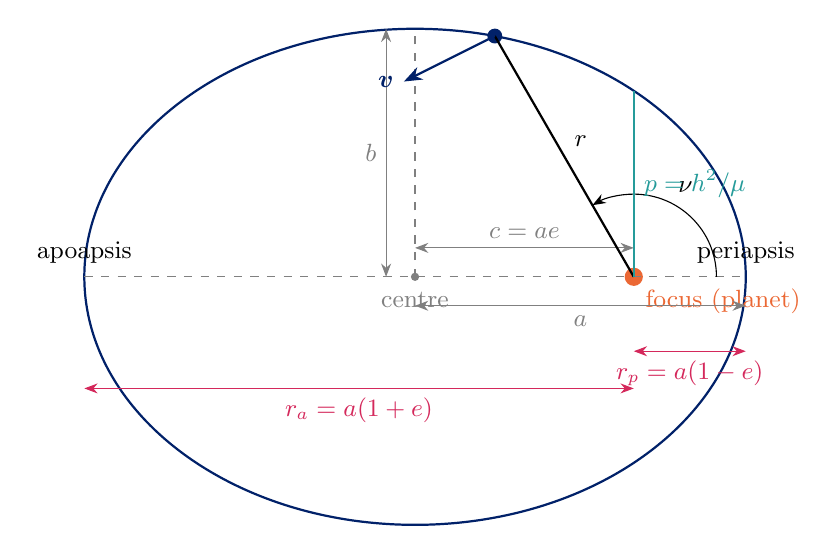
\begin{tikzpicture}[scale=1.05,>=Stealth]
  \def\a{4}\def\b{3}\def\c{2.6458}
  \draw[CUblue,thick] (0,0) ellipse ({\a} and {\b});
  \fill[sforange] (\c,0) circle (0.11) node[below right=1pt] {\small focus (planet)};
  \fill[gray] (0,0) circle (0.05) node[below=2pt] {\small centre};
  \draw[dashed,gray] (-\a,0) -- (\a,0);
  \draw[dashed,gray] (0,0) -- (0,\b);
  \draw[<->,gray] (0,-0.35) -- node[below] {\small $a$} (\a,-0.35);
  \draw[<->,gray] (-0.35,0) -- node[left] {\small $b$} (-0.35,\b);
  \draw[<->,gray] (0,0.35) -- node[above] {\small $c=ae$} (\c,0.35);
  % point P at nu = 120 deg
  \pgfmathsetmacro{\nuP}{120}
  \pgfmathsetmacro{\pp}{\b*\b/\a}
  \pgfmathsetmacro{\rP}{\pp/(1+0.66144*cos(\nuP))}
  \coordinate (P) at ({\c+\rP*cos(\nuP)},{\rP*sin(\nuP)});
  \fill[CUblue] (P) circle (0.09);
  \draw[thick] (\c,0) -- (P) node[midway,above right] {\small $r$};
  \draw[->] (\c+1.0,0) arc (0:\nuP:1.0);
  \node at ({\c+1.25*cos(\nuP/2)},{1.25*sin(\nuP/2)}) {\small $\nu$};
  % semi-latus rectum
  \draw[CUteal,thick] (\c,0) -- (\c,\pp) node[midway,right] {\small $p=h^2/\mu$};
  % periapsis / apoapsis
  \draw[<->,CUmagenta] (\c,-0.9) -- node[below] {\small $r_p=a(1-e)$} (\a,-0.9);
  \draw[<->,CUmagenta] (-\a,-1.35) -- node[below] {\small $r_a=a(1+e)$} (\c,-1.35);
  \node[above] at (\a,0.05) {\small periapsis};
  \node[above] at (-\a,0.05) {\small apoapsis};
  % velocity at P (perpendicular-ish to r for illustration)
  \draw[->,thick,CUblue] (P) -- ++(-1.1,-0.55) node[left] {\small $\bv v$};
\end{tikzpicture}
\caption{Geometry of an elliptical orbit ($e=0.66$). The planet sits at a focus, not the centre; $p$ is the radius at $\nu=90^\circ$.}
\label{fig:ellipse}
\end{figure}

\section{Speeds: circular, escape, hyperbolic}
From \cref{eq:visviva}:
\begin{equation}
  v_c=\sqrt{\frac{\mu}{r}}\ (a=r),\qquad
  v_{esc}=\sqrt{\frac{2\mu}{r}}=\sqrt2\,v_c\ (\En=0),\qquad
  v=\sqrt{\vinf^2+\frac{2\mu}{r}}\ (\En=\tfrac12\vinf^2>0).
  \label{eq:speeds}
\end{equation}
The third form---speed on a hyperbola at radius $r$ for a given excess speed---is the single most
used formula in interplanetary $\dv$ estimates. \Cref{fig:visviva} plots all three with an
elliptical example.

\begin{figure}[htb]\centering
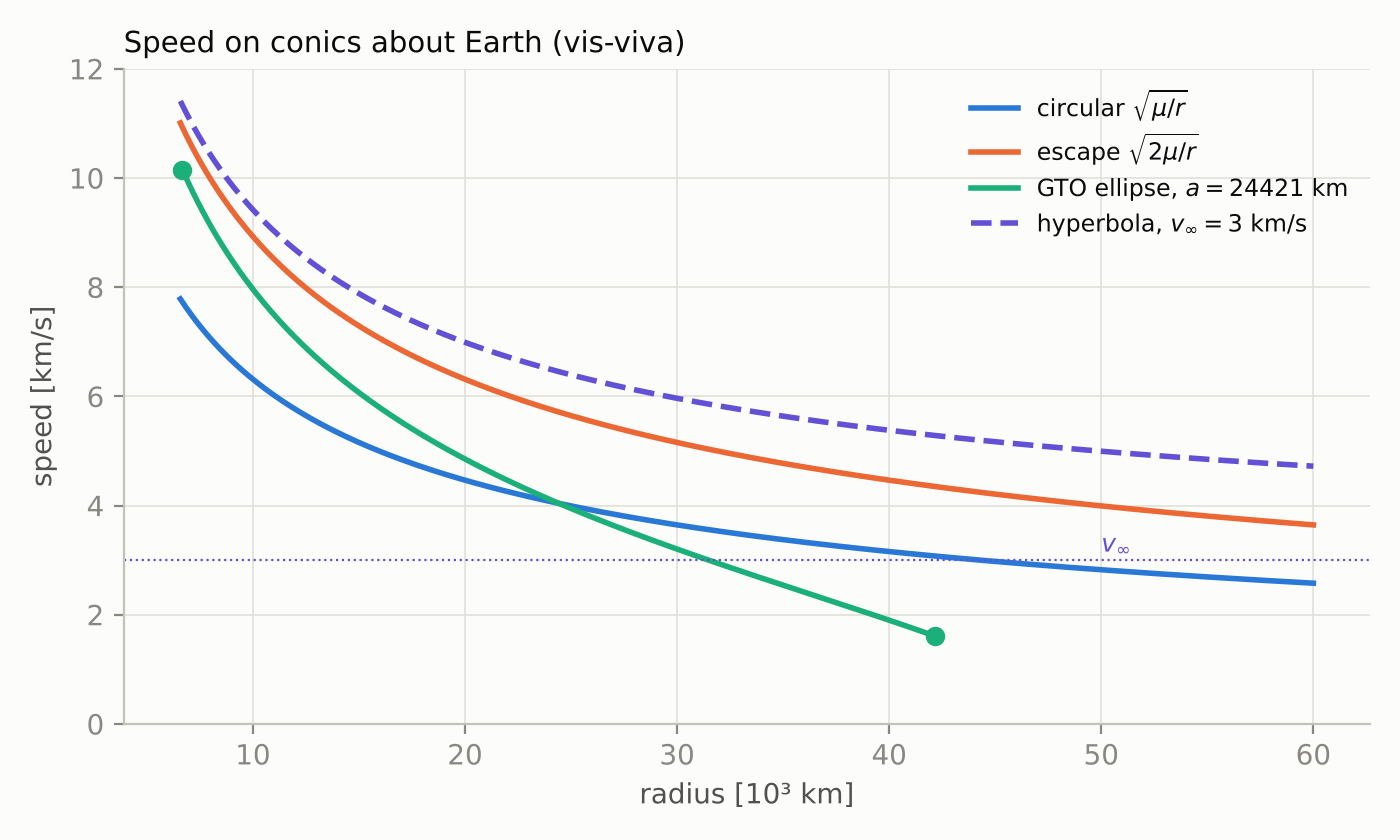
\includegraphics[width=0.78\textwidth]{tut_visviva}
\caption{Speed versus radius about Earth for circular, escape, an elliptical (GTO) and a hyperbolic orbit. Where the GTO curve crosses the circular curve is where a circular orbit of that radius has the same speed---nowhere useful; the ellipse is faster than circular at perigee and slower at apogee.}
\label{fig:visviva}
\end{figure}

\begin{worked}{ISS and GTO}
A 420-km circular orbit: $r=\SI{6798}{km}$, $v_c=\SI{\ISSvc}{km/s}$, period
$T=2\pi\sqrt{r^3/\mu}=\SI{\ISSperiodmin}{min}$, escape speed $\SI{\ISSvesc}{km/s}$,
$\En=\SI{\ISSenergy}{km^2/s^2}$.
A geostationary transfer orbit (GTO) with perigee 300~km and apogee 35,786~km: $a=\SI{\GTOa}{km}$,
$e=\GTOe$, $p=\SI{\GTOp}{km}$, $h=\SI{\GTOh}{km^2/s}$; perigee speed $\SI{\GTOvp}{km/s}$, apogee
speed $\SI{\GTOva}{km/s}$ (vis-viva at the two radii), period $\SI{\GTOperiodh}{h}$,
$\En=\SI{\GTOenergy}{km^2/s^2}$. Geostationary radius from $T=\SI{86164}{s}$:
$a=(\mu T^2/4\pi^2)^{1/3}=\SI{\GEOa}{km}$ (altitude \SI{\GEOalt}{km}), $v_c=\SI{\GEOvc}{km/s}$.
\end{worked}

\section{Time: Kepler's equation}
\Cref{eq:conic} gives shape, not timing. For an ellipse the period follows from $h=r^2\dot\nu$
integrated over one revolution (area $\pi ab$):
\begin{equation}
  T=2\pi\sqrt{\frac{a^3}{\mu}},\qquad n\equiv\frac{2\pi}{T}=\sqrt{\frac{\mu}{a^3}}\quad\text{(mean motion)}.
\end{equation}
To know \emph{where} the spacecraft is at time $t$ one introduces the \emph{mean anomaly}
$M=n(t-t_p)$ (an angle that grows uniformly with time, $t_p$ the periapsis passage) and the
\emph{eccentric anomaly} $E$ (an auxiliary angle measured from the ellipse's centre). They are linked by
\begin{keyresult}
\begin{equation}
  M=E-e\sin E\quad\text{(Kepler's equation)},\qquad
  \tan\frac{\nu}{2}=\sqrt{\frac{1+e}{1-e}}\,\tan\frac{E}{2},\qquad r=a(1-e\cos E).
  \label{eq:kepler}
\end{equation}
\end{keyresult}
Kepler's equation is transcendental: given $M$ it is solved for $E$ by Newton iteration
($E_{k+1}=E_k-(E_k-e\sin E_k-M)/(1-e\cos E_k)$), which converges in a handful of steps. For a
hyperbola the analogue is $M=e\sinh F-F$ with $r=a(1-e\cosh F)$. \Cref{fig:anomalies} shows the
effect: on an eccentric orbit the true anomaly races through periapsis and crawls through apoapsis.

\begin{figure}[htb]\centering
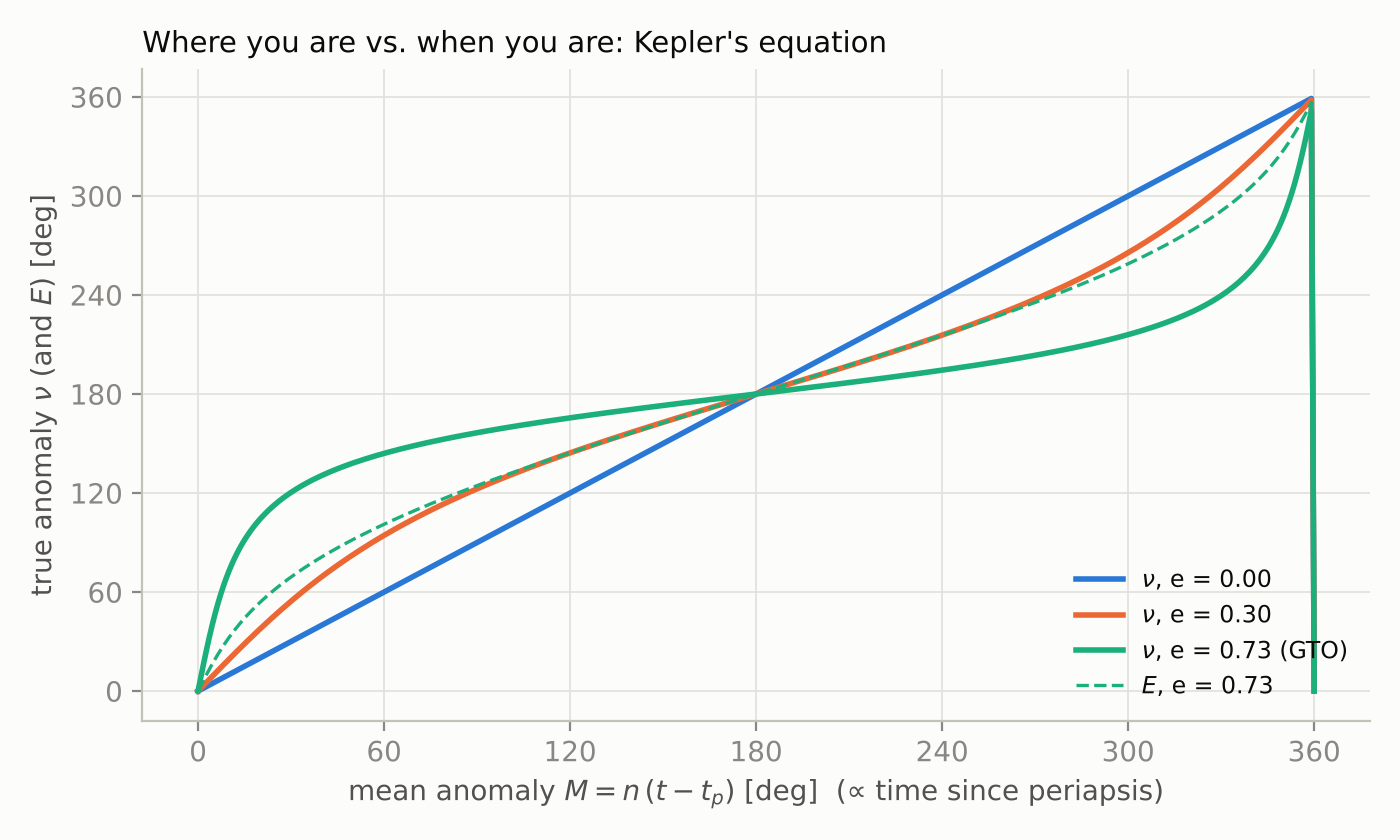
\includegraphics[width=0.78\textwidth]{tut_anomalies}
\caption{True anomaly (position) versus mean anomaly (time) for three eccentricities. On the GTO ($e=0.73$) the spacecraft covers the first $90^\circ$ of true anomaly in \SI{\GTOtninetymin}{min} of a \SI{\GTOperiodh}{h} period.}
\label{fig:anomalies}
\end{figure}

\begin{worked}{Time on the GTO}
From perigee to $\nu=90^\circ$ on the GTO above: $E=2\arctan\big(\sqrt{(1-e)/(1+e)}\tan 45^\circ\big)=\SI{\GTOEninety}{\degree}$,
$M=E-e\sin E=\SI{\GTOMninety}{\degree}$, $t=M/n=\SI{\GTOtninetymin}{min}$---against
\SI{\GTOhalfperiodmin}{min} for half the orbit. The spacecraft spends most of its time near apogee.
\end{worked}

\paragraph{Universal variables.} Code that must handle ellipses, parabolas and hyperbolas with
one formula uses the \emph{universal anomaly} $\chi$ and the Stumpff functions $C(z)$, $S(z)$ of
$z=\chi^2/a$; Kepler's equation becomes a single root-finding problem for all conics and the
position at time $t$ follows from the Lagrange coefficients $f,g$ (\cref{ch:lambert}). The
derivation is in Curtis Ch.~3 and Bate--Mueller--White Ch.~4; for this tutorial it is enough to
know that \code{propagate(r0, v0, dt, mu)} does exactly this.

\section{Orbits in three dimensions}
A conic in space needs six numbers (the \emph{classical orbital elements}): size $a$, shape $e$,
and three angles that orient the orbital plane and the periapsis---inclination $i$ of the plane
to the reference plane, right ascension of the ascending node $\Omega$ (where the orbit crosses
the reference plane going north), argument of periapsis $\omega$ (from the node to periapsis)---plus
the true anomaly $\nu$ for the position. The reference plane is the Earth's equator (J2000) for
Earth orbits and the ecliptic (Earth's orbital plane) for heliocentric work; the two are tilted by
the obliquity $23.44^\circ$. Converting a state vector $(\bv r,\bv v)$ to elements is a sequence of
cross and dot products ($\bv h=\bv r\times\bv v$, node vector $\bv N=\uv K\times\bv h$,
eccentricity vector from the derivation above); converting back rotates the in-plane
position $r(\cos\nu,\sin\nu)$ through $\omega$, $i$, $\Omega$. For mission analysis we spend most
of our time with magnitudes in a plane, but the three-dimensional machinery is what lets
\cref{ch:ephemeris,ch:lambert} place real planets in real frames.

\begin{codebox}
\code{kepler.py}: \code{vis\_viva}, \code{circular\_velocity}, \code{escape\_velocity},
\code{period}, \code{specific\_energy}; \code{kepler\_E}, \code{kepler\_H},
\code{time\_since\_periapsis}; \code{coe\_from\_rv}, \code{rv\_from\_coe} (elements $\leftrightarrow$ state);
\code{propagate} (universal-variable two-body propagation); hyperbola helpers
\code{hyperbolic\_periapsis\_speed}, \code{hyperbolic\_eccentricity}, \code{turn\_angle}.
\end{codebox}

\begin{pitfall}
The planet is at the \emph{focus}, so the distance from the planet to the orbit's centre is
$c=ae$, and periapsis radius is $a(1-e)$, not $a$. Altitude is radius minus the body radius;
forgetting to add $R$ when converting an altitude is the most common error in this subject.
\end{pitfall}

\subsection*{Exercises}
\begin{enumerate}[label=1.\arabic*,nosep]
\item Circular speed, period and escape speed for a 500-km orbit about Mars.
\item A burn at a 300-km Earth perigee raises speed by \SI{3.5}{km/s} above circular. Is the
      orbit bound? If not, what is $\vinf$ and $C_3=\vinf^2$?
\item On the GTO of the worked example, how long from perigee to apogee? Why is it exactly half the period regardless of $e$?
\end{enumerate}

%==================================================================
\chapter{Changing orbits: impulsive maneuvers}\label{ch:maneuvers}
%==================================================================

\section{The impulsive approximation}
A chemical burn of a few minutes on an orbit of ninety minutes (or of a few hours on a transfer of
months) can be idealized as an instantaneous change of velocity at fixed position: the
\emph{impulsive $\dv$}. Before the burn the spacecraft is on conic~1 at $\bv r$ with $\bv v_1$;
after it, on conic~2 at the same $\bv r$ with $\bv v_2$; the propulsion system must deliver
\begin{equation}
  \dv=|\bv v_2-\bv v_1| .
\end{equation}
The approximation fails when the burn is long compared with the time over which gravity
changes the velocity direction---low thrust-to-weight upper stages lose a few percent
(\emph{gravity loss}), electric propulsion is a different regime entirely (not covered here).

\begin{propulsion}
Mission analysis ends where propulsion design starts: the rocket equation $\zeta=m_p/m_0=1-e^{-\dv/c}$
with $c=\gz\Isp$ (\cref{ch:staging}). A budget of \SI{5.7}{km/s} is \SI{\ZetaThreeTwoZero}{} of the
initial mass in propellant at $\Isp=\SI{320}{s}$ and \SI{\ZetaFourFiveZero}{} at \SI{450}{s}. Every
\SI{100}{m/s} saved in this tutorial is worth about 3\% of the stage's initial mass---that is
why the subject is worth a propulsion engineer's time.
\end{propulsion}

\section{Energy per unit \texorpdfstring{$\dv$}{dv}: the Oberth effect}
Differentiating \cref{eq:energy} at fixed $r$: $\dd\En=\bv v\cdot\dd\bv v$. A given $\dv$ changes
the orbital energy most when it is applied \emph{along} the velocity and where the velocity is
\emph{largest}---at periapsis. The same propellant buys more energy deep in a gravity well. This
is the Oberth effect and it decides where interplanetary injections and captures are performed
(\cref{sec:departure}).

\section{The Hohmann transfer}
Between two coplanar circular orbits of radii $r_1<r_2$ the two-impulse transfer of minimum
total $\dv$ is the ellipse tangent to both: periapsis $r_1$, apoapsis $r_2$, $a_t=(r_1+r_2)/2$.
With vis-viva on the three orbits,
\begin{keyresult}
\begin{align}
  v_{c,1}&=\sqrt{\mu/r_1}, & v_{t,p}&=\sqrt{\mu\Big(\frac{2}{r_1}-\frac{1}{a_t}\Big)}, & \dv_1&=v_{t,p}-v_{c,1},\\
  v_{c,2}&=\sqrt{\mu/r_2}, & v_{t,a}&=\sqrt{\mu\Big(\frac{2}{r_2}-\frac{1}{a_t}\Big)}, & \dv_2&=v_{c,2}-v_{t,a},
\end{align}
\begin{equation}
  t_H=\pi\sqrt{a_t^3/\mu}\quad\text{(half the transfer-orbit period)}.
\end{equation}
\end{keyresult}
Both burns are tangential (no direction change), which is why the transfer is cheap. Normalized
by $v_{c,1}$ the total depends only on $r_2/r_1$ (\cref{fig:hohmann}): it rises to a maximum of
$\HohPeakValue\,v_{c,1}$ at $r_2/r_1=\HohPeakRatio$ and then \emph{falls} toward the escape value
$\sqrt2-1=\HohEscapeLimit$---raising an orbit to a very high circular altitude costs more than
leaving altogether. For $r_2/r_1\gtrsim 12$ a three-impulse bi-elliptic transfer (out to a high
intermediate apoapsis and back) beats Hohmann slightly, at the cost of a much longer flight.

\begin{figure}[htb]\centering
\begin{minipage}[c]{0.36\textwidth}\centering
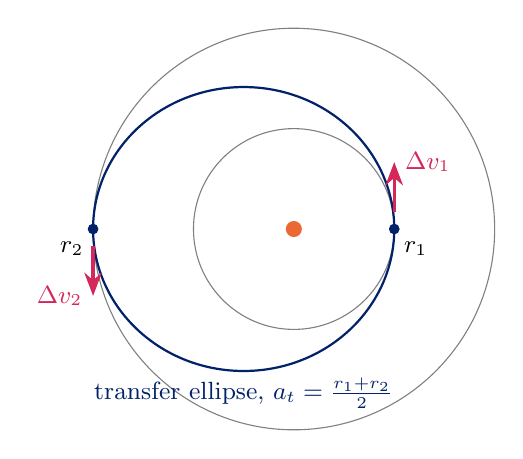
\begin{tikzpicture}[scale=0.85,>=Stealth]
  \draw[gray] (0,0) circle (1.5); \draw[gray] (0,0) circle (3);
  \fill[sforange] (0,0) circle (0.12);
  \draw[CUblue,thick] (-0.75,0) ellipse (2.25 and 2.1213);
  \fill[CUblue] (1.5,0) circle (0.08); \fill[CUblue] (-3,0) circle (0.08);
  \draw[->,CUmagenta,very thick] (1.5,0.25) -- (1.5,1.0) node[right] {\small $\dv_1$};
  \draw[->,CUmagenta,very thick] (-3,-0.25) -- (-3,-1.0) node[left] {\small $\dv_2$};
  \node[below right] at (1.5,-0.05) {\small $r_1$}; \node[below left] at (-3,-0.05) {\small $r_2$};
  \node[CUblue] at (-0.75,-2.45) {\small transfer ellipse, $a_t=\frac{r_1+r_2}{2}$};
\end{tikzpicture}
\end{minipage}\hfill
\begin{minipage}[c]{0.62\textwidth}\centering
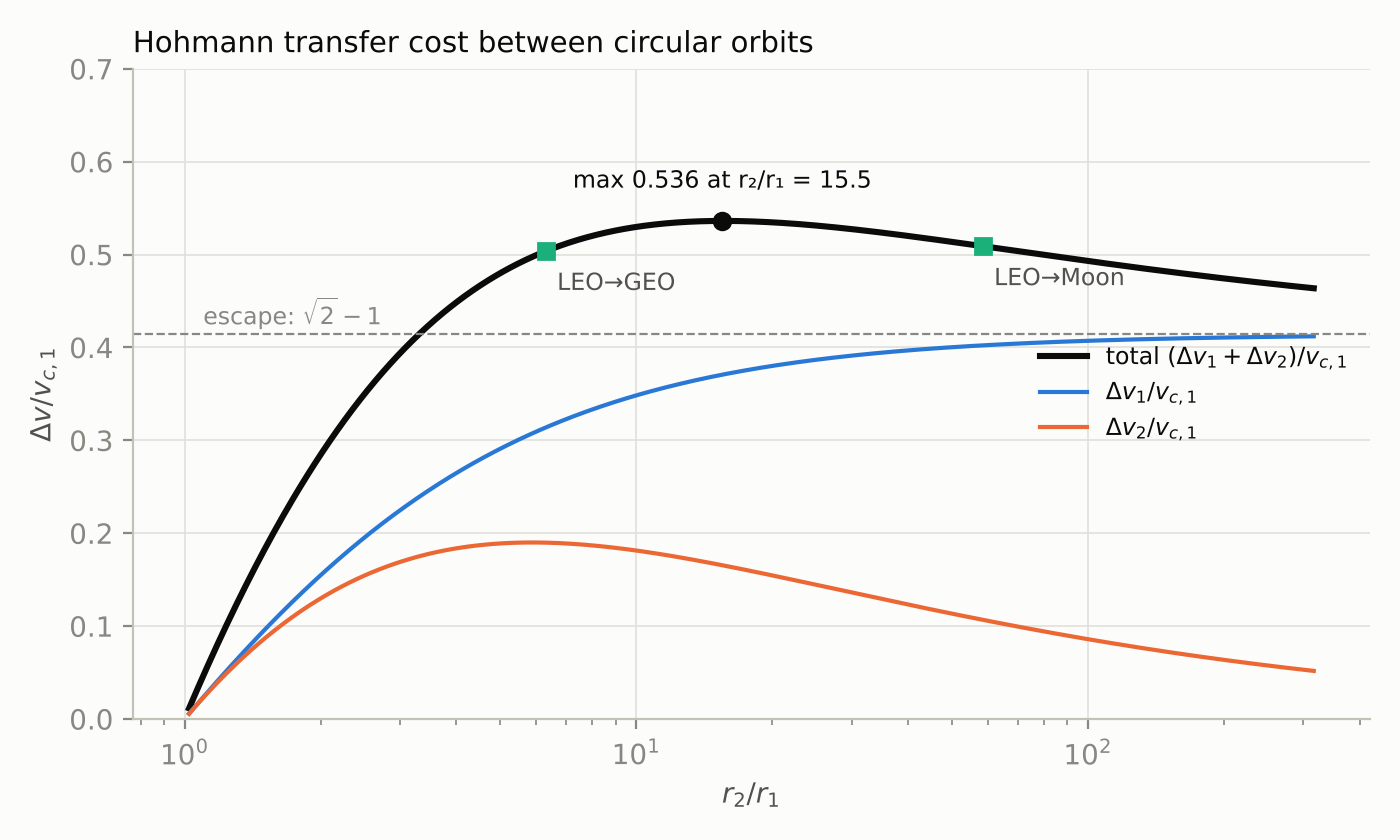
\includegraphics[width=\linewidth]{tut_hohmann_norm}
\end{minipage}
\caption{Left: Hohmann geometry; both burns are along the velocity. Right: normalized cost versus radius ratio, with the maximum at $r_2/r_1\approx\HohPeakRatio$ and the escape limit.}
\label{fig:hohmann}
\end{figure}

\begin{worked}{LEO to GEO}
$r_1=\SI{6678}{km}$ (300~km), $r_2=\SI{\GEOa}{km}$: $v_{c,1}=\SI{\HohLEOGEOvcone}{km/s}$,
$v_{t,p}=\SI{\HohLEOGEOvtp}{km/s}$, $\dv_1=\SI{\HohLEOGEOdvone}{km/s}$; $v_{t,a}=\SI{\HohLEOGEOvta}{km/s}$,
$v_{c,2}=\SI{\HohLEOGEOvctwo}{km/s}$, $\dv_2=\SI{\HohLEOGEOdvtwo}{km/s}$; total
\SI{\HohLEOGEOtot}{km/s}, $t_H=\SI{\HohLEOGEOtofh}{h}$.
Bi-elliptic check at $r_2/r_1=15$ with an intermediate apoapsis of $60r_1$: \SI{\BiEllTot}{km/s}
against Hohmann's \SI{\BiEllHoh}{km/s}, but \SI{\BiEllTOFd}{days} instead of \SI{\BiEllHohTOFh}{h}.
\end{worked}

\section{Plane changes}
Rotating the velocity vector by $\Delta i$ at constant speed costs
\begin{equation}
  \dv=2v\sin\frac{\Delta i}{2},
\end{equation}
which is proportional to $v$: do plane changes where the spacecraft is slowest. Combining a plane
change with a speed change in one burn costs
$\dv=\sqrt{v_1^2+v_2^2-2v_1v_2\cos\Delta i}$, less than the two done separately. For LEO$\to$GEO
from a launch site at latitude $28.5^\circ$ (which fixes the minimum inclination,
\cref{ch:launch}) the \SI{28.5}{\degree} plane change costs \SI{\PCatLEO}{km/s} if done in LEO,
\SI{\PCatGEO}{km/s} if done at GEO, and the optimal split---\SI{\HohPCdione}{\degree} at the
perigee burn, \SI{\HohPCditwo}{\degree} at the apogee burn---brings the total transfer to
\SI{\HohPCtot}{km/s} against \SI{\HohLEOGEOtot}{km/s} without plane change.

\section{Phasing: when to go}
A Hohmann transfer only arrives at the target if the target is there. The target must lead the
departure point by the angle it will \emph{not} cover during the flight,
\begin{equation}
  \phi_{lead}=\pi-n_2\,t_H,
\end{equation}
and this geometry repeats every \emph{synodic period} $S$, $1/S=1/T_1-1/T_2$. For Earth--Mars:
$\phi_{lead}=\SI{\PhaseEM}{\degree}$ and $S=\SI{\SynEM}{days}$ (2.14~yr). This is why Mars
launch windows come every 26 months and why ``when'' is as much a design variable as ``how fast''.

\begin{codebox}
\code{transfers.py}: \code{hohmann}, \code{bielliptic}, \code{plane\_change\_dv}, \code{combined\_dv},
\code{hohmann\_with\_plane\_change} (optimal split by 1-D minimization), \code{synodic\_period},
\code{hohmann\_phase\_angle}, \code{wait\_for\_phase}, \code{hohmann\_round\_trip}.
\end{codebox}

\begin{pitfall}
$\dv$ is a vector difference. Adding magnitudes is only right when the two velocities are
parallel (tangential burns). A plane change of $60^\circ$ costs a full $v$---as much as
the orbital speed itself.
\end{pitfall}

\subsection*{Exercises}
\begin{enumerate}[label=2.\arabic*,nosep]
\item Hohmann transfer from a 400-km Earth orbit to the Moon's distance (\SI{384400}{km}), treating the Moon as absent: $\dv_1$, $\dv_2$ to circularize there, and $t_H$. Compare $\dv_1$ with the TLI of \cref{ch:moon}.
\item Why does $\dv_2/v_{c,1}$ in \cref{fig:hohmann} peak and then decrease with $r_2/r_1$?
\item Show that combining a plane change with the apogee burn of a GTO is cheaper than doing it at perigee, using the numbers of the worked example.
\end{enumerate}

%==================================================================
\chapter{Leaving one body for another: patched conics}\label{ch:patched}
%==================================================================

\section{Spheres of influence}
With the Sun, a planet and a spacecraft we have a three-body problem, which has no closed-form
solution. The engineering escape is to notice that near a planet the planet's gravity dominates,
far from it the Sun's does, and to \emph{patch} two-body conics at the boundary. Laplace's sphere
of influence (SOI), the radius where the planet's perturbation of the heliocentric motion equals
the Sun's perturbation of the planetocentric motion, is
\begin{equation}
  r_{SOI}=a\Big(\frac{m}{M}\Big)^{2/5},
\end{equation}
with $a$ the planet's orbital radius and $m/M$ its mass ratio to the Sun. Values:
Venus \SI{\SOIVenus e3}{km}, Earth \SI{\SOIEarth e3}{km} ($=\SI{\SOIEarthAU}{AU}$,
$145R_\oplus$), Mars \SI{\SOIMars e3}{km}, Jupiter \SI{\SOIJupiter e3}{km}, Saturn
\SI{\SOISaturn e3}{km}; the Moon about Earth \SI{\SOIMoon e3}{km}. Two consequences:
on the heliocentric scale Earth's SOI is a point (\SI{0.6}{\percent} of an AU), so the
spacecraft ``leaves Earth'' at Earth's position with Earth's velocity plus whatever
excess velocity it has; on the planetocentric scale the SOI is effectively infinity
(\num{145} Earth radii), so the planetocentric conic can be treated as reaching $r\to\infty$.
The SOI radius itself never appears in a $\dv$ formula---only the two limits do.

\begin{figure}[htb]\centering
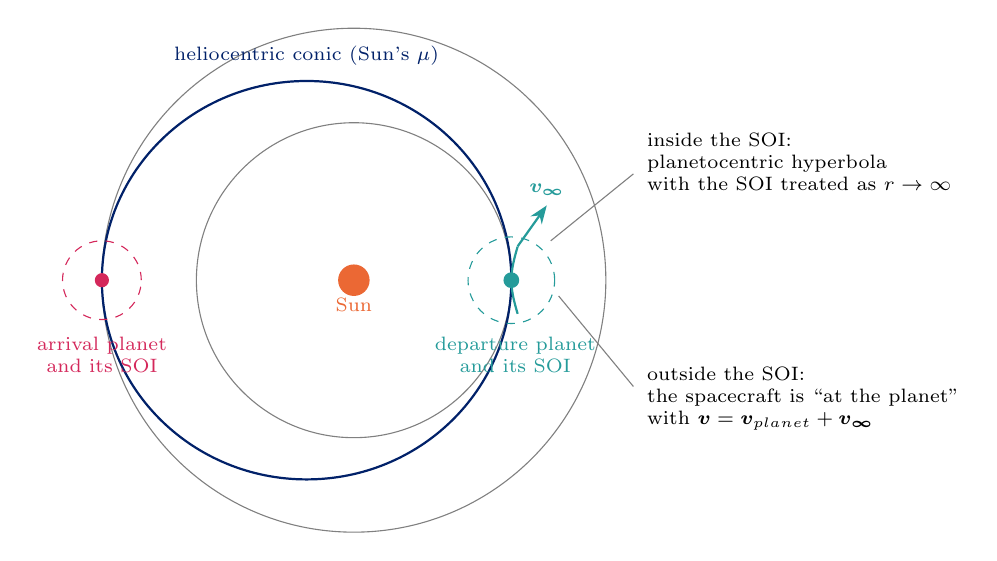
\begin{tikzpicture}[scale=1.0,>=Stealth]
  \fill[sforange] (0,0) circle (0.2) node[below=3pt,font=\scriptsize] {Sun};
  \draw[gray] (0,0) circle (2); \draw[gray] (0,0) circle (3.2);
  \draw[CUblue,thick] (-0.6,0) ellipse (2.6 and 2.53);
  \fill[CUteal] (2,0) circle (0.1); \draw[CUteal,dashed] (2,0) circle (0.55);
  \fill[CUmagenta] (-3.2,0) circle (0.09); \draw[CUmagenta,dashed] (-3.2,0) circle (0.5);
  \node[CUteal,font=\scriptsize,align=center] at (2.05,-0.95) {departure planet\\and its SOI};
  \node[CUmagenta,font=\scriptsize,align=center] at (-3.2,-0.95) {arrival planet\\and its SOI};
  \node[CUblue,font=\scriptsize] at (-0.6,2.85) {heliocentric conic (Sun's $\mu$)};
  % hyperbola sketch inside departure SOI, periapsis near the planet
  \draw[CUteal,thick] plot[domain=-1.1:1.1,samples=40] ({2+0.12*cosh(\x)-0.12},{0.32*sinh(\x)});
  \draw[->,CUteal,thick] (2.08,0.43) -- (2.45,0.95) node[above,font=\scriptsize] {$\bv\vinf$};
  \node[align=left,font=\scriptsize,anchor=west] at (3.6,1.5) {inside the SOI:\\planetocentric hyperbola\\with the SOI treated as $r\to\infty$};
  \node[align=left,font=\scriptsize,anchor=west] at (3.6,-1.5) {outside the SOI:\\the spacecraft is ``at the planet''\\with $\bv v=\bv v_{planet}+\bv\vinf$};
  \draw[gray,thin] (3.55,1.35) -- (2.5,0.5); \draw[gray,thin] (3.55,-1.35) -- (2.6,-0.2);
\end{tikzpicture}
\caption{The patched-conic idea: a heliocentric conic between the planets' positions, and a planetocentric hyperbola inside each sphere of influence, matched through $\bv\vinf$.}
\label{fig:patched}
\end{figure}

\section{Departure: from parking orbit to hyperbola}\label{sec:departure}
Suppose the heliocentric leg requires the spacecraft to leave Earth's SOI with velocity
$\bv\vinf$ relative to Earth (how we find it is the subject of \cref{sec:helio,ch:lambert}).
Inside the SOI the spacecraft is on a hyperbola of energy $\En=\vinf^2/2$. If it starts in a
circular parking orbit of radius $r_p$ and burns tangentially at the point that becomes the
hyperbola's periapsis, \cref{eq:speeds} gives
\begin{keyresult}
\begin{equation}
  \dv_{dep}=\sqrt{\vinf^2+\frac{2\mu}{r_p}}-\sqrt{\frac{\mu}{r_p}},\qquad C_3\equiv\vinf^2 .
  \label{eq:departure}
\end{equation}
\end{keyresult}
$C_3$ (\si{km^2/s^2}) is the quantity launch providers quote: a launch vehicle's performance curve is
payload mass versus $C_3$. The hyperbola's eccentricity, turning angle and asymptote direction
(\cref{fig:hyperbola}) are
\begin{equation}
  e=1+\frac{r_p\vinf^2}{\mu},\qquad \delta=2\arcsin\frac1e,\qquad \beta=\arccos\frac1e,
  \qquad \Delta=r_p\sqrt{1+\frac{2\mu}{r_p\vinf^2}},
\end{equation}
where $\beta$ is the angle from the periapsis direction to the outgoing asymptote (it tells you
where on the parking orbit to burn so that $\bv\vinf$ points the right way) and $\Delta$ is the
aiming radius---the lateral offset of the incoming asymptote from the planet's centre, used to
target a flyby.

\begin{figure}[htb]\centering
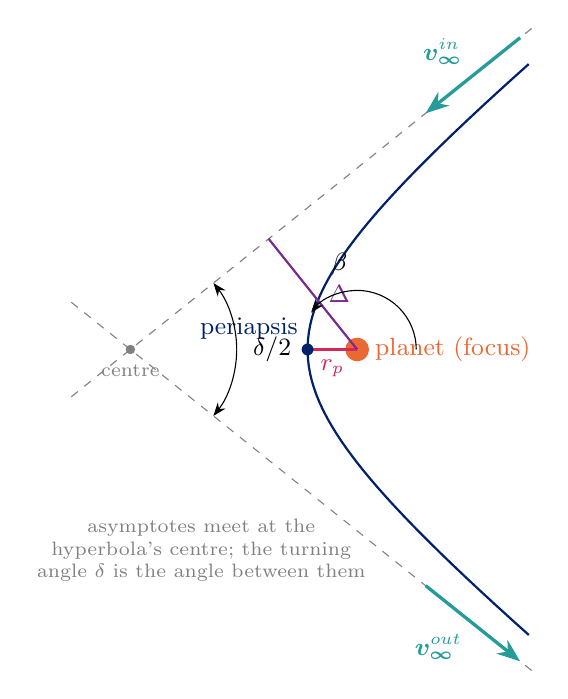
\begin{tikzpicture}[scale=1.5,>=Stealth]
  \def\a{1.5}\def\b{1.2}\def\c{1.92}
  \draw[dashed,gray] (-0.5,-0.4) -- (3.4,2.72); \draw[dashed,gray] (-0.5,0.4) -- (3.4,-2.72);
  \draw[CUblue,thick] plot[domain=-1.45:1.45,samples=60] ({\a*cosh(\x)},{\b*sinh(\x)});
  \fill[sforange] (\c,0) circle (0.1) node[right=3pt] {\small planet (focus)};
  \fill[gray] (0,0) circle (0.04) node[below=2pt,font=\scriptsize,gray] {centre};
  \draw[CUmagenta,thick] (\a,0) -- (\c,0) node[midway,below] {\small $r_p$};
  \fill[CUblue] (\a,0) circle (0.05) node[above left] {\small periapsis};
  \draw[->,very thick,CUteal] (3.3,2.64) -- (2.5,2.0) node[midway,above left] {\small $\bv\vinf^{in}$};
  \draw[->,very thick,CUteal] (2.5,-2.0) -- (3.3,-2.64) node[midway,below left] {\small $\bv\vinf^{out}$};
  \draw[CUpurple,thick] (\c,0) -- ({\c-0.8*0.9375},{0.9375}) node[midway,right=2pt] {\small $\Delta$};
  \draw[->] (0.9,0) arc (0:38.66:0.9); \draw[->] (0.9,0) arc (0:-38.66:0.9);
  \node at (1.2,0.0) {\small $\delta/2$};
  \draw[->] (\c+0.5,0) arc (0:141.3:0.5); \node at (\c-0.15,0.72) {\small $\beta$};
  \node[font=\scriptsize,align=center,gray] at (0.6,-1.7) {asymptotes meet at the\\hyperbola's centre; the turning\\angle $\delta$ is the angle between them};
\end{tikzpicture}
\caption{Hyperbolic passage ($e=1.28$): incoming and outgoing asymptotes, turning angle $\delta=2\arcsin(1/e)$, angle $\beta=\arccos(1/e)$ from periapsis to the outgoing asymptote, periapsis radius $r_p$ and aiming radius $\Delta$.}
\label{fig:hyperbola}
\end{figure}

\begin{figure}[htb]\centering
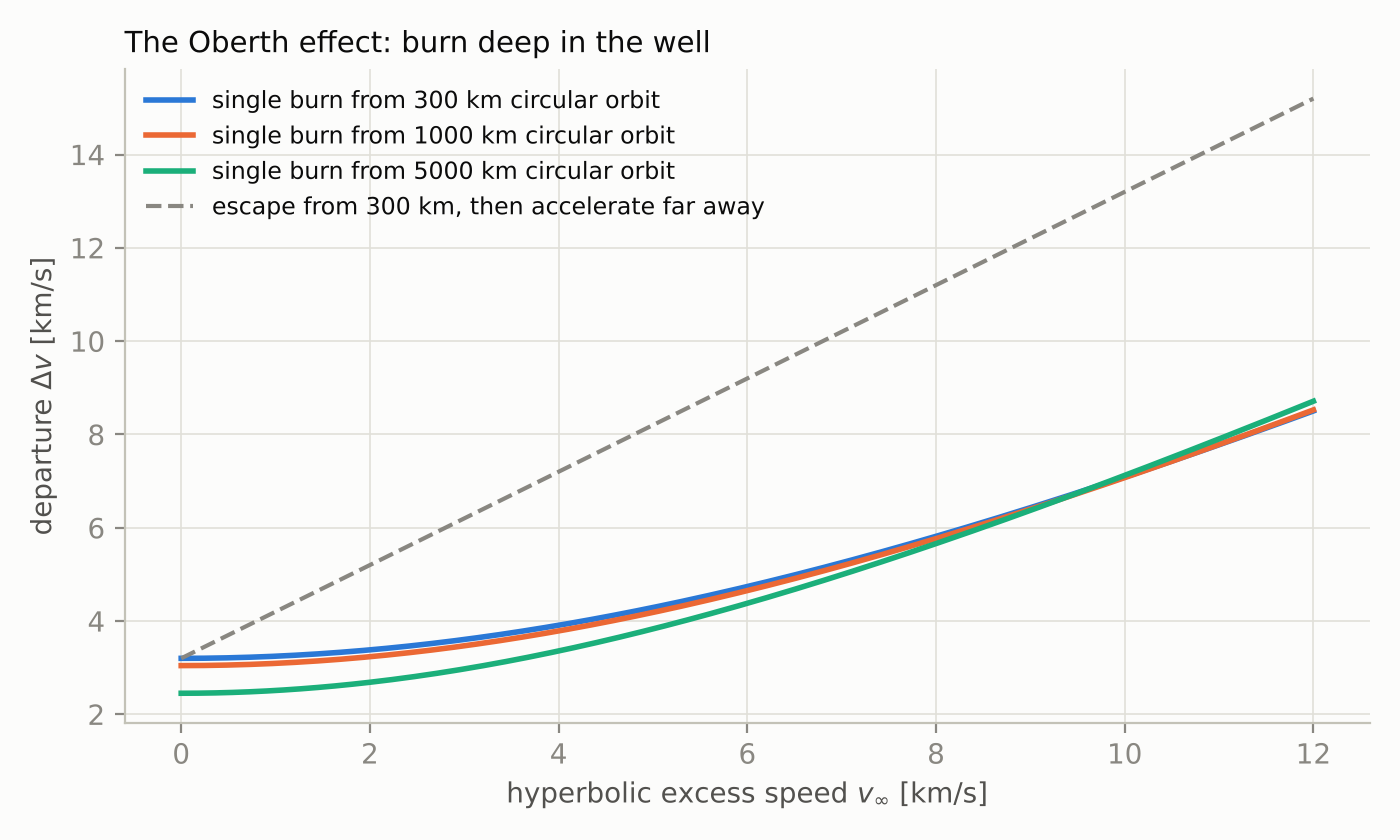
\includegraphics[width=0.7\textwidth]{tut_oberth}
\caption{Departure $\dv$ from a parking orbit versus $\vinf$ (\cref{eq:departure}) compared with escaping first and accelerating later---the Oberth effect.}
\label{fig:oberth}
\end{figure}

\begin{worked}{Oberth in numbers}
To leave Earth with $\vinf=\SI{\Obvinf}{km/s}$ from a 300-km orbit ($v_c=\SI{\EMvpark}{km/s}$,
$v_{esc}=\SI{\ObvescLEO}{km/s}$): a single tangential burn costs
$\dv=\sqrt{3^2+2\mu/r_p}-v_c=\SI{\Obdv}{km/s}$. Escaping first (\SI{\Obesc}{km/s}) and
then accelerating to \SI{3}{km/s} far from Earth would cost \SI{6.2}{km/s}. The \SI{3}{km/s} of
excess speed is bought for \SI{0.4}{km/s} because it is added where the spacecraft already moves
at \SI{11}{km/s} (\cref{fig:oberth}).
\end{worked}

\section{Arrival: capture}
Arriving with excess speed $\vinf$, the spacecraft is on a hyperbola. To stay it must burn at
periapsis $r_p$ from the hyperbolic speed down to the speed of the desired orbit:
\begin{keyresult}
\begin{equation}
  \dv_{cap}=\sqrt{\vinf^2+\frac{2\mu}{r_p}}-\sqrt{\mu\Big(\frac{2}{r_p}-\frac{2}{r_p+r_a}\Big)} .
  \label{eq:capture}
\end{equation}
\end{keyresult}
Capturing into a \emph{high ellipse} ($r_a\gg r_p$) is much cheaper than circularizing, because
the elliptical periapsis speed is close to the hyperbolic one; the remaining circularization can
be left to repeated apoapsis-lowering burns or to aerobraking (\cref{ch:aero}). For circular
capture there is an optimal periapsis: minimizing \cref{eq:capture} with $r_a=r_p$ over $r_p$ gives
$r_p^{*}=2\mu/\vinf^2$ (\cref{fig:capture})---at Mars with $\vinf=\SI{\EMvinfarr}{km/s}$ that is an
altitude of \SI{\EMcapOptAlt}{km}, far above where science orbits are, so in practice one captures
low into an ellipse.

\begin{figure}[htb]\centering
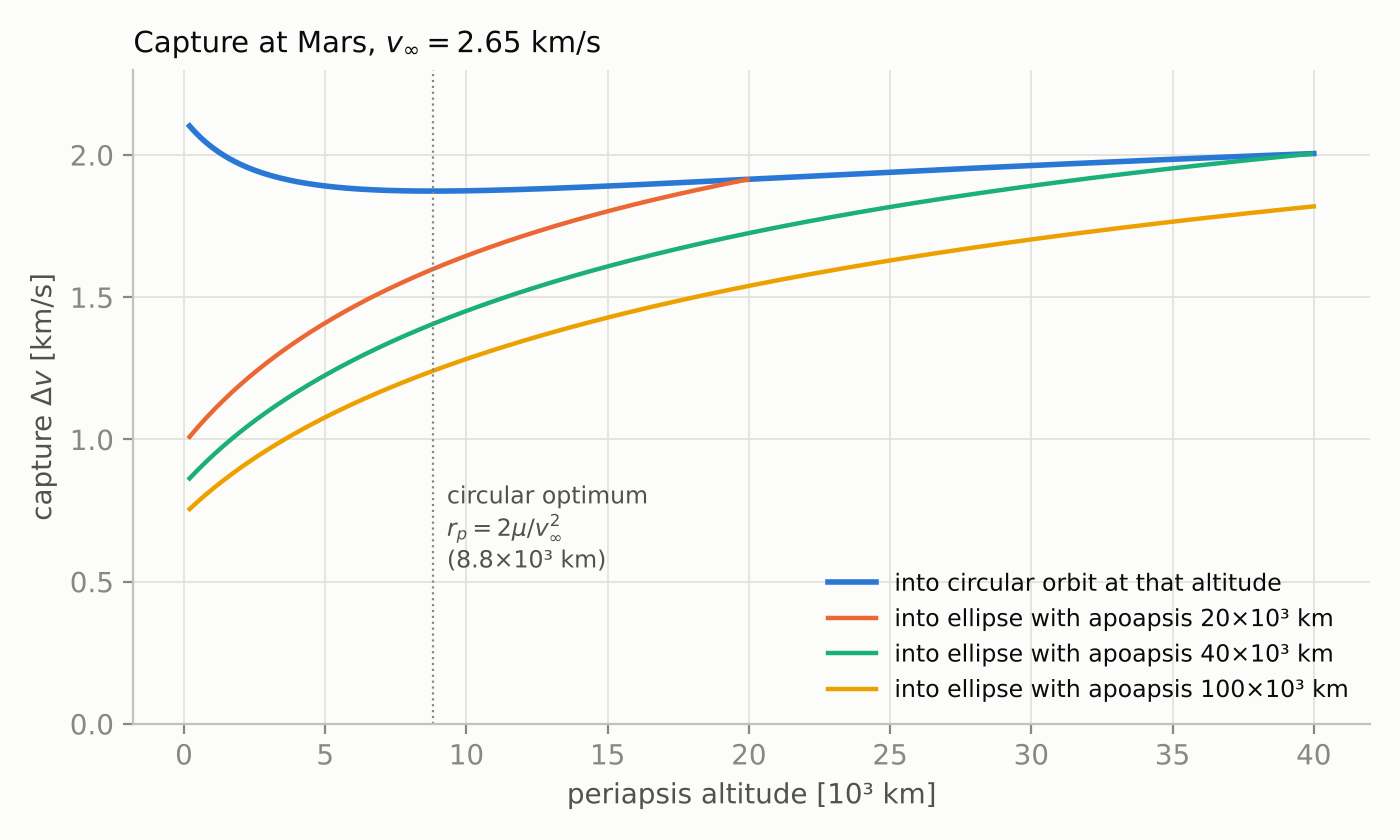
\includegraphics[width=0.72\textwidth]{tut_capture}
\caption{Capture $\dv$ at Mars versus periapsis altitude for circular and elliptical capture orbits.}
\label{fig:capture}
\end{figure}

\section{The heliocentric leg: Hohmann between planets}\label{sec:helio}
Treat the planets' orbits as coplanar circles of radii $a_1$, $a_2$ about the Sun. The Hohmann
ellipse between them has perihelion speed $v_{t,p}$ and aphelion speed $v_{t,a}$
(\cref{ch:maneuvers} with $\mu_\odot$). The planets move at $v_1=\sqrt{\mu_\odot/a_1}$ and
$v_2=\sqrt{\mu_\odot/a_2}$ along the same directions, so the required excess speeds are simply
\begin{equation}
  \vinf^{dep}=v_{t,p}-v_1,\qquad \vinf^{arr}=v_2-v_{t,a}.
\end{equation}
These feed \cref{eq:departure,eq:capture}. \Cref{tab:planets} gives the result for four targets;
these are the ``textbook'' numbers against which any dated mission (\cref{ch:lambert}) should be checked.

\begin{worked}{Earth to Mars, textbook}
$v_{t,p}=\SI{\EMvtp}{km/s}$ vs.\ Earth's \SI{\EMvEarth}{km/s} $\Rightarrow\vinf^{dep}=\SI{\EMvinfdep}{km/s}$
($C_3=\SI{\EMCthree}{km^2/s^2}$); $v_{t,a}=\SI{\EMvta}{km/s}$ vs.\ Mars's \SI{\EMvMars}{km/s}
$\Rightarrow\vinf^{arr}=\SI{\EMvinfarr}{km/s}$; $t_H=\SI{\EMtofd}{days}$.
Departure from a 300-km orbit: hyperbolic periapsis speed \SI{\EMvhyp}{km/s}, $\dv=\SI{\EMdvdep}{km/s}$,
$e=\EMehyp$, $\beta=\SI{\EMturnhalf}{\degree}$. Capture at Mars into a 400-km circular orbit:
hyperbolic speed \SI{\EMcapvhyp}{km/s}, circular \SI{\EMcapvc}{km/s}, $\dv=\SI{\EMcapcirc}{km/s}$;
into a $400\times\SI{40000}{km}$ ellipse: $\dv=\SI{\EMcapell}{km/s}$.
\end{worked}

\begin{table}[htb]\centering\small
\caption{Hohmann (circular, coplanar) transfers from Earth, departure from a 300-km parking orbit.}
\label{tab:planets}
\begin{tabular}{lcccccccc}\toprule
Target & $\vinf^{dep}$ [km/s] & $C_3$ [km$^2$/s$^2$] & $\dv_{dep}$ [km/s] & $\vinf^{arr}$ [km/s] & $t_H$ [d] & lead angle & synodic [yr] \\\midrule
Venus & \PlVenusvinfdep & \PlVenusCthree & \PlVenusdvdep & \PlVenusvinfarr & \PlVenustofd & $\PlVenusphase^\circ$ & \PlVenussyn \\
Mars & \PlMarsvinfdep & \PlMarsCthree & \PlMarsdvdep & \PlMarsvinfarr & \PlMarstofd & $\PlMarsphase^\circ$ & \PlMarssyn \\
Jupiter & \PlJupitervinfdep & \PlJupiterCthree & \PlJupiterdvdep & \PlJupitervinfarr & \PlJupitertofd & $\PlJupiterphase^\circ$ & \PlJupitersyn \\
Saturn & \PlSaturnvinfdep & \PlSaturnCthree & \PlSaturndvdep & \PlSaturnvinfarr & \PlSaturntofd & $\PlSaturnphase^\circ$ & \PlSaturnsyn \\\bottomrule
\end{tabular}
\end{table}

\section{Gravity assists}
Inside a planet's SOI the spacecraft's speed relative to the planet is the same on the way in
and out ($|\bv\vinf^{in}|=|\bv\vinf^{out}|$: energy is conserved in the planet frame), but its
direction is rotated by the turning angle $\delta$. In the \emph{Sun's} frame the velocity is
$\bv v=\bv v_{planet}+\bv\vinf$, and because $\bv\vinf$ has rotated, $|\bv v|$ changes
(\cref{fig:ga}). The free heliocentric speed change is
\begin{keyresult}
\begin{equation}
  |\dv_{helio}|=|\bv\vinf^{out}-\bv\vinf^{in}|=2\vinf\sin\frac{\delta}{2}=\frac{2\vinf}{1+r_p\vinf^2/\mu}.
\end{equation}
\end{keyresult}
For a fixed closest approach $r_p$ this is largest when $\vinf=\sqrt{\mu/r_p}$---the circular speed
at the flyby radius---and the maximum equals that speed. Passing \emph{behind} the planet (trailing
side) adds energy; passing in front subtracts it. The momentum comes from the planet, whose
orbit changes immeasurably. When the heliocentric legs before and after the flyby demand
$\bv\vinf$ vectors of different magnitude, the mismatch is made up by a small burn at periapsis
(a \emph{powered flyby}); \code{flyby\_powered} finds the shared periapsis radius from the
required turning and charges the speed difference.

\begin{figure}[htb]\centering
\begin{minipage}[c]{0.4\textwidth}\centering
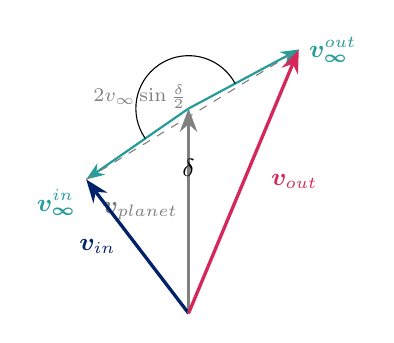
\begin{tikzpicture}[scale=1.0,>=Stealth]
  \coordinate (O) at (0,0);
  \coordinate (Vp) at (0,2.6);
  \draw[->,very thick,gray] (O) -- (Vp) node[midway,left] {\small $\bv v_{planet}$};
  \coordinate (Vin) at ($(Vp)+(-1.3,-0.9)$);
  \coordinate (Vout) at ($(Vp)+(1.4,0.75)$);
  \draw[->,thick,CUteal] (Vp) -- (Vin) node[below left] {\small $\bv\vinf^{in}$};
  \draw[->,thick,CUteal] (Vp) -- (Vout) node[right] {\small $\bv\vinf^{out}$};
  \draw[->,very thick,CUblue] (O) -- (Vin) node[midway,left=4pt] {\small $\bv v_{in}$};
  \draw[->,very thick,CUmagenta] (O) -- (Vout) node[midway,right=6pt] {\small $\bv v_{out}$};
  \draw[dashed,gray] (Vin) -- (Vout) node[midway,above left=-2pt] {\scriptsize $2\vinf\sin\frac{\delta}{2}$};
  \draw (Vp) ++(-0.55,-0.38) arc (214.7:28.2:0.67); \node at ($(Vp)+(0.0,-0.75)$) {\small $\delta$};
\end{tikzpicture}
\end{minipage}\hfill
\begin{minipage}[c]{0.58\textwidth}\centering
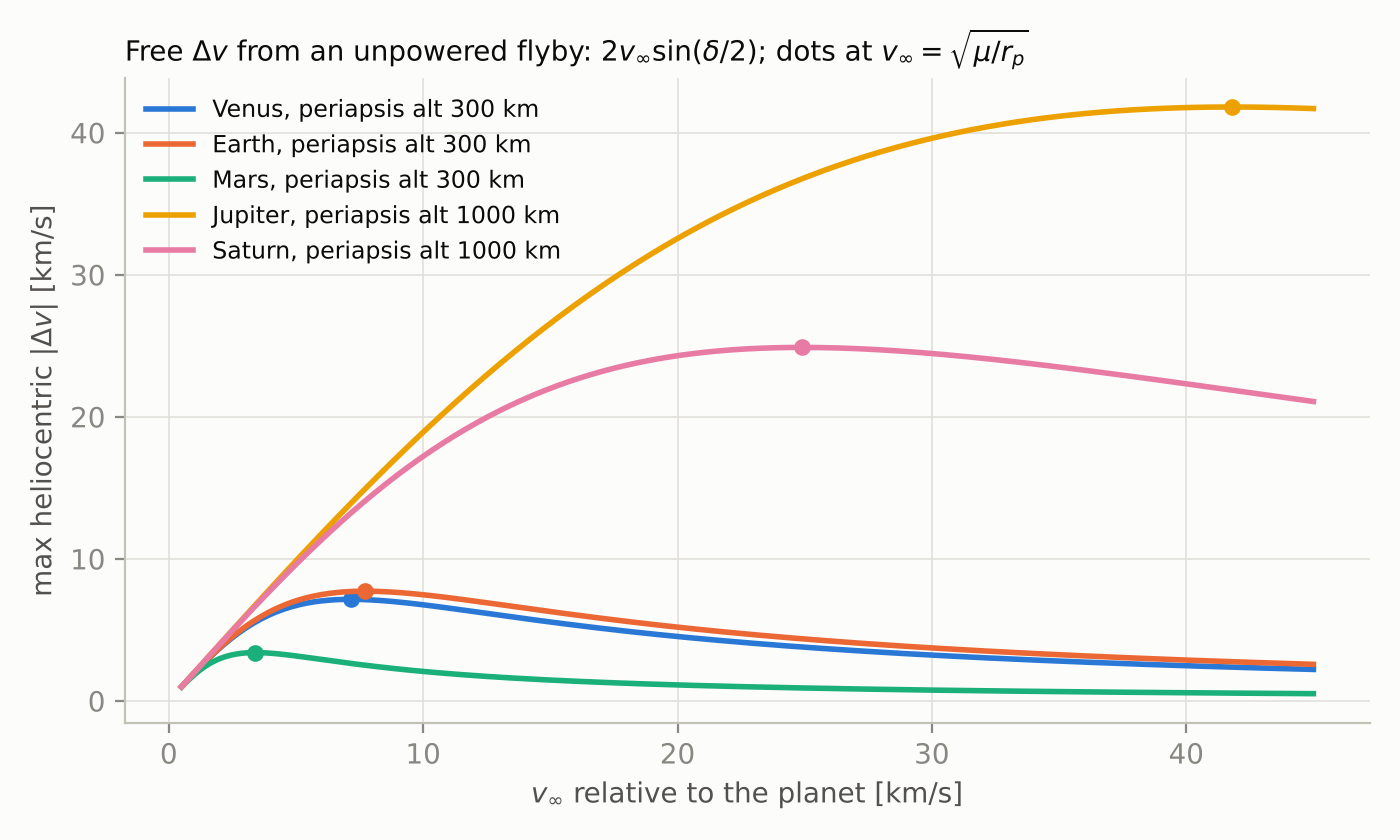
\includegraphics[width=\linewidth]{tut_gravity_assist}
\end{minipage}
\caption{Left: in the planet frame $\bv\vinf$ rotates by $\delta$ at constant magnitude; adding $\bv v_{planet}$ gives a longer heliocentric velocity. Right: maximum free $\dv$ versus $\vinf$ for five planets at a fixed closest approach.}
\label{fig:ga}
\end{figure}

\begin{worked}{Voyager 2 at Jupiter}
Using only the launch (1977-08-20), Jupiter (1979-07-09) and Saturn (1981-08-25) dates and the
ephemeris of \cref{ch:ephemeris}, the Earth--Jupiter and Jupiter--Saturn legs (\cref{ch:lambert})
give $\vinf^{in}=\SI{\Vgvinfin}{km/s}$ and $\vinf^{out}=\SI{\Vgvinfout}{km/s}$ at Jupiter, a
required turning of \SI{\Vgturn}{\degree}, a closest approach of \SI{\Vgrp e3}{km} (the real
flyby was about \SI{650e3}{km} from the centre), and a heliocentric speed change from
\SI{\Vgvin}{km/s} to \SI{\Vgvout}{km/s}---\SI{\Vghelio}{km/s} for a powered correction of only
\SI{\Vgdvpow}{km/s}. Launch $C_3$ was \SI{\VgCthree}{km^2/s^2}.
\end{worked}

\begin{codebox}
\code{patched\_conics.py}: \code{departure\_dv}, \code{capture\_dv}, \code{optimal\_capture\_periapsis},
\code{flyby\_unpowered}, \code{flyby\_powered}, \code{flyby\_max\_heliocentric\_dv},
\code{hohmann\_interplanetary} (\cref{tab:planets}), \code{heliocentric\_leg},
\code{interplanetary\_mission} (a whole sequence of bodies and dates). SOI radii: \code{Body.soi}.
\end{codebox}

\begin{pitfall}
$\vinf$ is a velocity \emph{relative to the planet}; $C_3$ is its square. A heliocentric speed is
never a $\vinf$. And the departure $\dv$ is \emph{not} $\vinf$: it is \cref{eq:departure}, which for
small $\vinf$ is close to the escape burn $(\sqrt2-1)v_c$.
\end{pitfall}

\subsection*{Exercises}
\begin{enumerate}[label=3.\arabic*,nosep]
\item Jupiter arrival with the Hohmann $\vinf$ of \cref{tab:planets}: capture $\dv$ into a 1000-km circular orbit, and into a $1000\times\SI{2e6}{km}$ ellipse. Where is the circular optimum?
\item A Venus flyby at 300-km altitude with $\vinf=\SI{5}{km/s}$: eccentricity, turning angle, maximum heliocentric $\dv$.
\item Explain with \cref{fig:ga} why a flyby cannot change $|\bv\vinf|$ but can change the spacecraft's heliocentric energy.
\end{enumerate}

%==================================================================
\chapter{Where are the planets? Ephemerides}\label{ch:ephemeris}
%==================================================================
\Cref{ch:patched} assumed circular coplanar planetary orbits. Real missions launch on calendar
dates, so we need planet positions and velocities as functions of time: an \emph{ephemeris}.

\section{Mean elements and secular rates}
A planet's orbit is nearly Keplerian; the other planets perturb its elements slowly. Over a few
centuries the drift is well represented by linear trends, and JPL publishes exactly such a table
(\emph{Keplerian Elements for Approximate Positions of the Major Planets}): for each planet six
elements at the epoch J2000 and six rates per Julian century, valid 1800--2050 (a second table
extends to 3000~BC--3000~AD). The algorithm is the inverse of \cref{ch:twobody}:
\begin{enumerate}[nosep]
\item $T=(JD_{TT}-2451545.0)/36525$ centuries since J2000;
\item $a, e, i, L, \varpi, \Omega$ each $=x_0+\dot x\,T$ (the table uses mean longitude $L$ and
      longitude of perihelion $\varpi$; then $\omega=\varpi-\Omega$ and $M=L-\varpi$);
\item solve Kepler's equation for $E$, then $\nu$ and $r$ (\cref{eq:kepler});
\item rotate the in-plane position and velocity through $\omega$, $i$, $\Omega$ into the J2000 ecliptic frame.
\end{enumerate}
The result is good to tens of arcseconds for the inner planets and a few arcminutes for Saturn
(JPL's own statement, confirmed in the package tests against an independent model). In velocity
terms the error is of order \SI{1}{m/s} at Earth---negligible for $\dv$ budgets, unusable for
navigation.

\begin{worked}{Mars on the day of the lecture (2026-11-12)}
$T=\EphT$ centuries. Mars: $a=\SI{\EphMarsa}{AU}$, $e=\EphMarse$, $M=\SI{\EphMarsM}{\degree}$,
$\nu=\SI{\EphMarsnu}{\degree}$; heliocentric distance \SI{\EphrMars}{AU}, speed \SI{\EphvMars}{km/s},
ecliptic longitude \SI{\EphLonMars}{\degree}. Earth: \SI{\EphrEarth}{AU}, \SI{\EphvEarth}{km/s},
longitude \SI{\EphLonEarth}{\degree}. Mars leads Earth by \SI{\EphPhase}{\degree}---more than the
Hohmann lead angle of \SI{\PhaseEM}{\degree}, so the ideal departure date is \emph{just past}; the
porkchop plot of \cref{ch:lambert} confirms the window is open. Earth--Mars distance \SI{\EphdistEM}{AU}.
\end{worked}

\section{Frames, the Moon and time}
Planet positions are referred to the J2000 ecliptic; Earth-centric work (launch azimuths, the
declination of a departure asymptote) uses the J2000 equator, a rotation by the obliquity
$23.439^\circ$ about the $x$-axis. The table's ``Earth'' is the Earth--Moon barycenter, which
Earth itself orbits with an amplitude of \SI{4700}{km}; the package can correct for this. The
Moon's geocentric position comes from a truncated Meeus series (dozens of periodic terms in the
Moon's mean anomaly, elongation and argument of latitude): on 2026-11-12 the Moon is
\SI{\EphMoonDist}{km} from Earth moving at \SI{\EphMoonSpeed}{km/s}; its distance ranges
363,000--406,000~km over a month, which matters for lunar-transfer $\dv$ at the \SI{10}{m/s}
level. Epochs are Julian Dates; the ephemeris wants Terrestrial Time, which runs \SI{69}{s} ahead
of UTC---an offset far below the accuracy of mean elements.

\begin{codebox}
\code{ephemeris.py}: \code{planet\_elements}, \code{planet\_state}, \code{earth\_state}
(barycenter correction), \code{moon\_state\_geocentric}, \code{body\_state} (any body, one call),
\code{heliocentric\_longitude}, \code{phase\_angle}, \code{to\_jd}, \code{jd\_to\_iso}.
\end{codebox}

\begin{pitfall}
Mean elements are not osculating elements: the planet's instantaneous velocity is computed from
the two-body relation on the \emph{mean} orbit, which is what makes the model consistent with the
Lambert solver that follows. Mixing in a precise ephemeris for one body and mean elements for
another buys nothing.
\end{pitfall}

%==================================================================
\chapter{Lambert's problem and porkchop plots}\label{ch:lambert}
%==================================================================

\section{The problem}
Given two position vectors $\bv r_1$, $\bv r_2$ about a central body and a time of flight
$\Delta t$, find the conic that connects them---i.e.\ the velocities $\bv v_1$ at departure and
$\bv v_2$ at arrival. This is Lambert's problem, and it is the workhorse of mission analysis
because the calendar, not the Hohmann geometry, fixes where the planets are: a departure on a
given date and an arrival on another date defines $\bv r_1$ (Earth then), $\bv r_2$ (Mars then)
and $\Delta t$. The Hohmann transfer is the special case where the two positions happen to be
$180^\circ$ apart and $\Delta t=t_H$.

\section{Geometry}
The transfer angle $\Delta\theta$ between $\bv r_1$ and $\bv r_2$ is either $<180^\circ$
(\emph{type I}, the ``short way'') or $>180^\circ$ (\emph{type II}, the ``long way''); for a
spacecraft that must move in the same sense as the planets (prograde), the sign of
$(\bv r_1\times\bv r_2)_z$ decides which. Exactly at $\Delta\theta=180^\circ$ the two positions and
the focus are collinear and the transfer plane is undefined---this singularity shows up as a
ridge in every porkchop plot. For a given geometry the ellipse of minimum energy has
$a_{min}=(r_1+r_2+c)/4$, $c$ the chord; longer flights use larger ellipses, shorter ones
hyperbolas.

\section{How it is solved}
Position and velocity at two times on the same conic are related by the Lagrange coefficients,
\begin{equation}
  \bv r_2=f\,\bv r_1+g\,\bv v_1,\qquad \bv v_2=\dot f\,\bv r_1+\dot g\,\bv v_1,
\end{equation}
so once $f$ and $g$ are known, $\bv v_1=(\bv r_2-f\bv r_1)/g$ and $\bv v_2=(\dot g\bv r_2-\bv r_1)/g$.
In the universal-variable formulation $f$, $g$, $\dot g$ and the time of flight all depend on
the geometry and on one unknown $z=\chi^2/a$ (negative for hyperbolas, zero for the parabola,
positive for ellipses) through the Stumpff functions $C(z)$, $S(z)$:
\begin{equation}
  A=\sin\Delta\theta\sqrt{\frac{r_1r_2}{1-\cos\Delta\theta}},\quad
  y(z)=r_1+r_2+A\,\frac{zS(z)-1}{\sqrt{C(z)}},\quad
  \sqrt\mu\,\Delta t=\Big[\frac{y}{C}\Big]^{3/2}S+A\sqrt y ,
  \label{eq:lambert}
\end{equation}
\begin{equation}
  f=1-\frac{y}{r_1},\qquad g=A\sqrt{\frac{y}{\mu}},\qquad \dot g=1-\frac{y}{r_2}.
\end{equation}
The time of flight is a monotonic function of $z$ on the single-revolution branch
(\cref{fig:lambert}), so solving Lambert's problem is a one-dimensional root find: bracket $z$
between a hyperbolic value and $z\to4\pi^2$ (the one-full-revolution limit) and let Brent's method
converge. This formulation never diverges, costs \SI{55}{\micro s} per solve and handles all conics
with one code path---the reasons it was chosen for the package.

\begin{figure}[htb]\centering
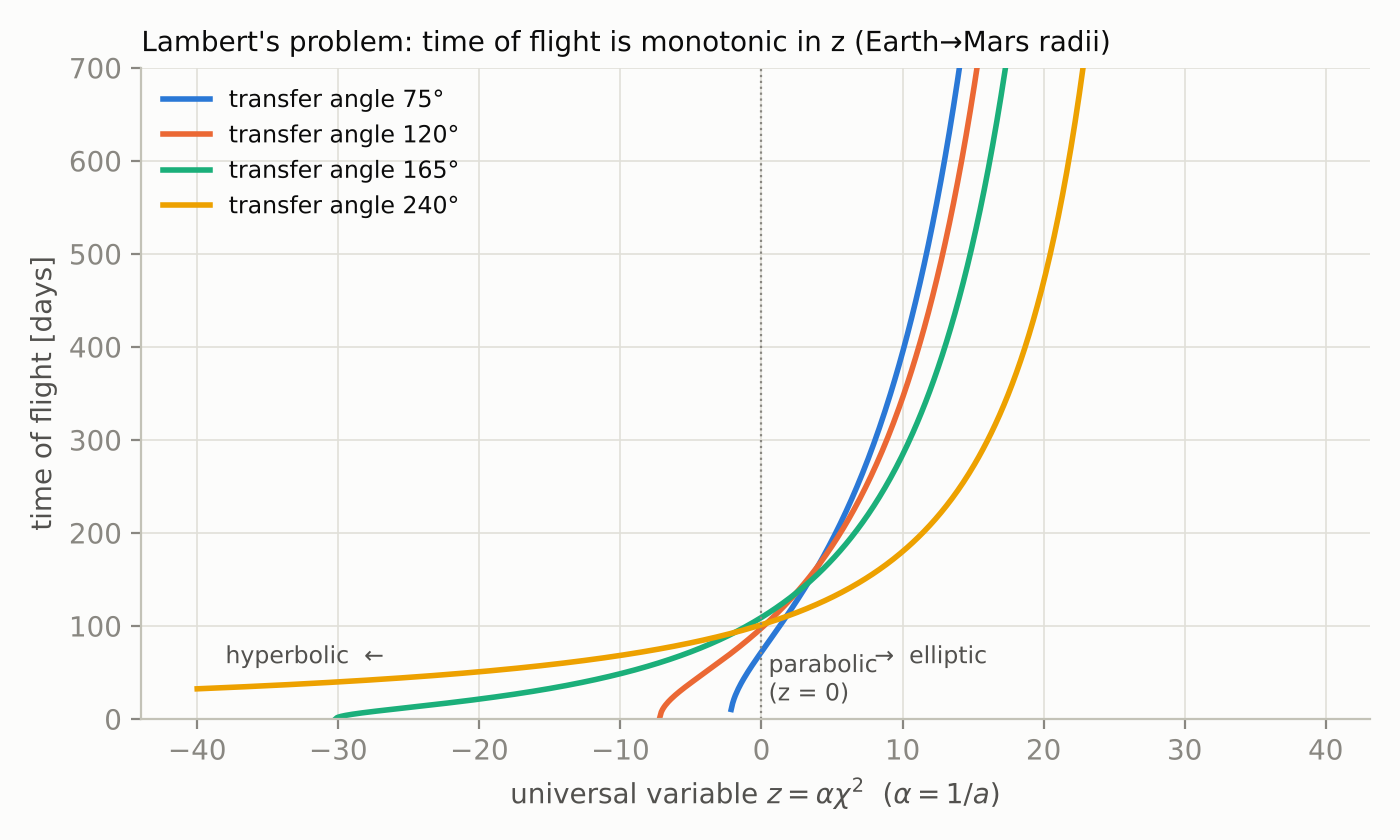
\includegraphics[width=0.72\textwidth]{tut_lambert_tof}
\caption{Time of flight versus the universal variable $z$ for Earth--Mars radii and four transfer angles. Given $\Delta t$, the solver finds the $z$ (hence the conic) by a bracketed root find.}
\label{fig:lambert}
\end{figure}

\section{From a Lambert solution to mission quantities}
With $\bv v_1$ and $\bv v_2$ in hand and the planets' velocities from the ephemeris,
\begin{equation}
  \bv\vinf^{dep}=\bv v_1-\bv v_{planet,1},\qquad \bv\vinf^{arr}=\bv v_2-\bv v_{planet,2},
\end{equation}
and \cref{eq:departure,eq:capture} give the burns. The $z$-component of $\bv\vinf^{dep}$ in the
equatorial frame is the declination of the launch asymptote (DLA), which must be reachable from
the launch site (\cref{ch:launch}).

\begin{worked}{A dated Earth--Mars transfer}
Depart 2026-10-30, arrive 2027-09-06 ($\Delta t=\SI{\Lamtofd}{days}$). Earth at \SI{\LamrOneAU}{AU}
moving at \SI{\LamvE}{km/s}; Mars at \SI{\LamrTwoAU}{AU}; transfer angle \SI{\Lamdtheta}{\degree}
(type II); transfer ellipse $a=\SI{\Lama}{AU}$; $|\bv v_1|=\SI{\LamvOne}{km/s}$. Then
$\vinf^{dep}=\SI{\Lamvinfdep}{km/s}$ ($C_3=\SI{\LamCthree}{km^2/s^2}$), $\vinf^{arr}=\SI{\Lamvinfarr}{km/s}$,
departure $\dv$ from 300~km \SI{\Lamdvdep}{km/s}, capture into 400~km circular \SI{\Lamdvcap}{km/s}.
Compare the textbook Hohmann values of \cref{ch:patched}: the real geometry costs a few percent more.
\end{worked}

\section{Porkchop plots}
Repeat the Lambert solution over a grid of departure dates and times of flight and contour the
result: a \emph{porkchop plot} (\cref{fig:porkchop}). Reading one is a core skill:
\begin{itemize}[nosep]
\item the two lobes are type I (below the ridge, shorter flights) and type II (above it);
\item the ridge between them is the $180^\circ$ singularity;
\item $C_3$ contours (what the launch vehicle must provide) and arrival $\vinf$ contours (what the
      capture system must absorb) have different optima---a mission chooses a compromise;
\item the width of the ``bowl'' at an acceptable $\dv$ is the \emph{launch window}; it recurs
      every synodic period with a different shape, because the planets' eccentric, inclined
      orbits make some oppositions better than others.
\end{itemize}

\begin{figure}[htb]\centering
\begin{minipage}[c]{0.6\textwidth}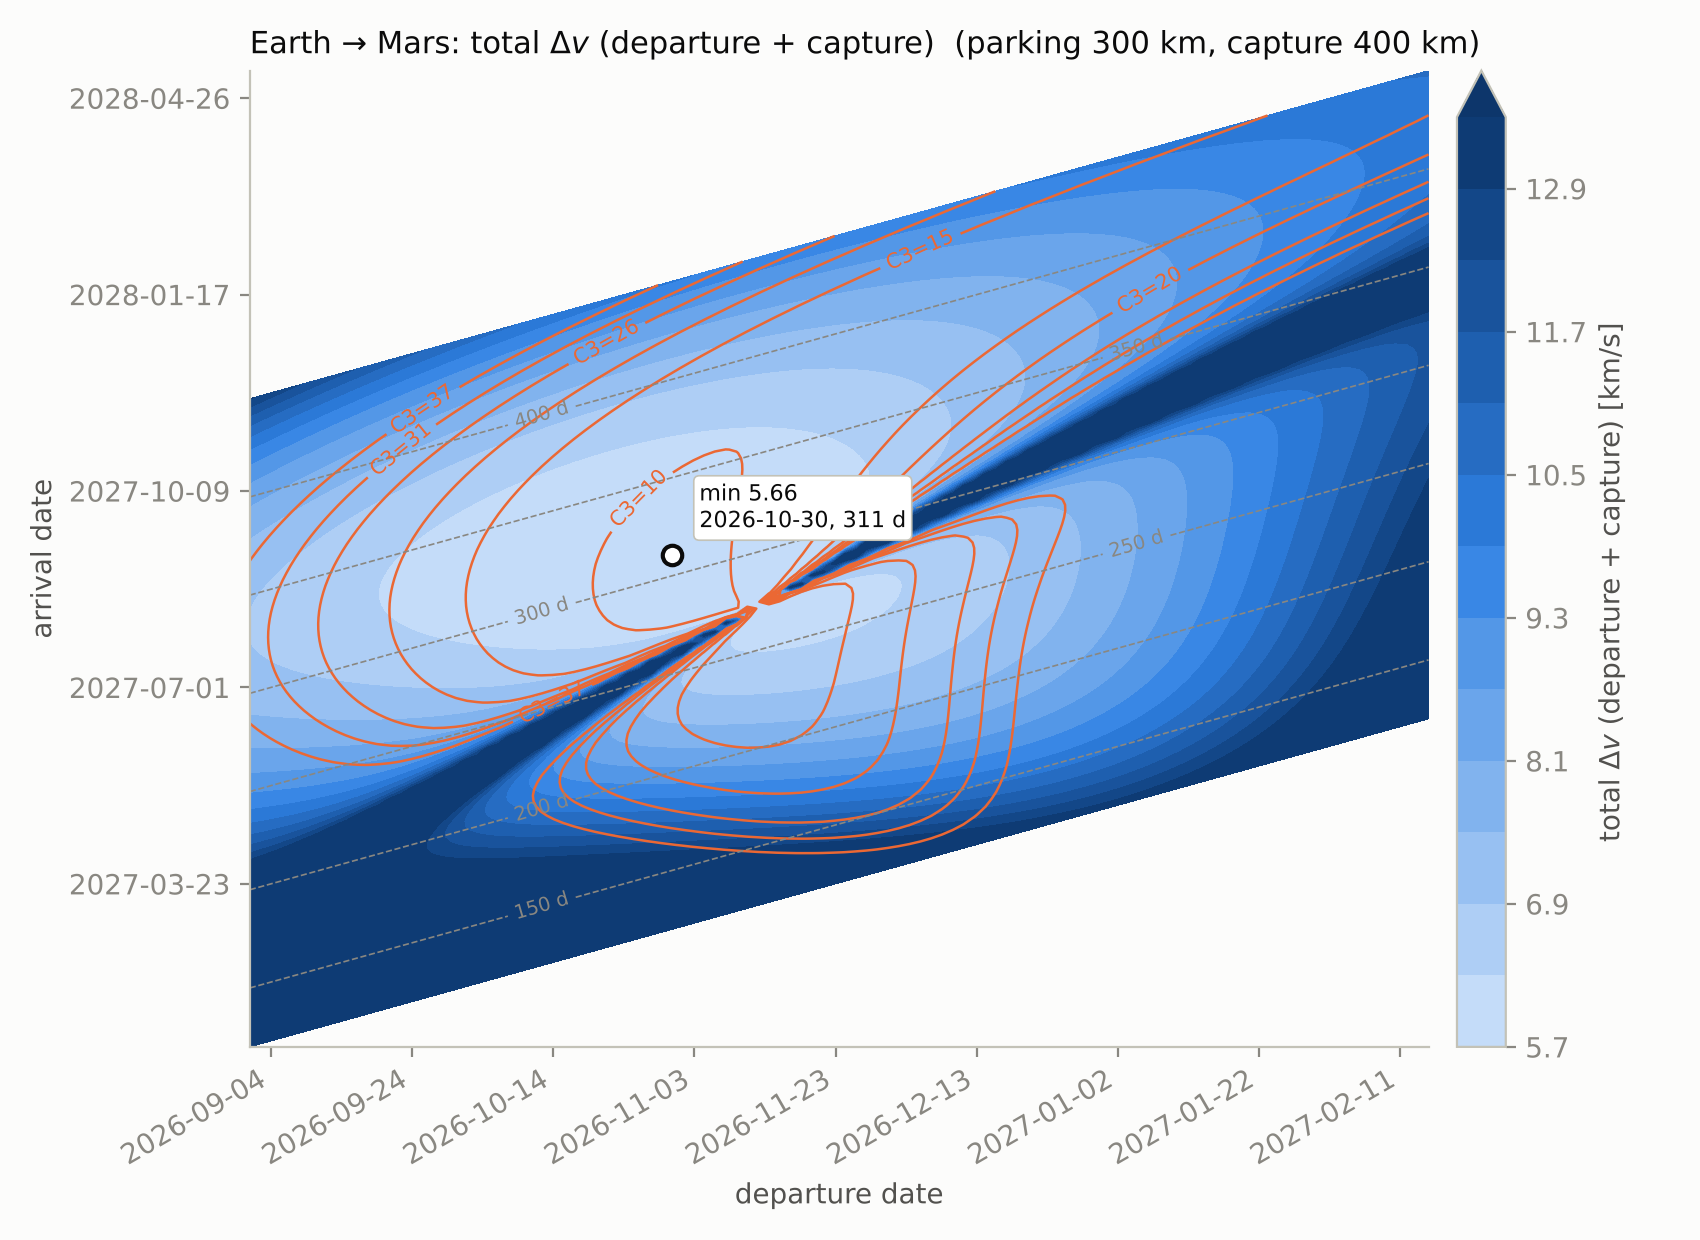
\includegraphics[width=\linewidth]{porkchop_earth_mars_2026_dvtotal}\end{minipage}\hfill
\begin{minipage}[c]{0.38\textwidth}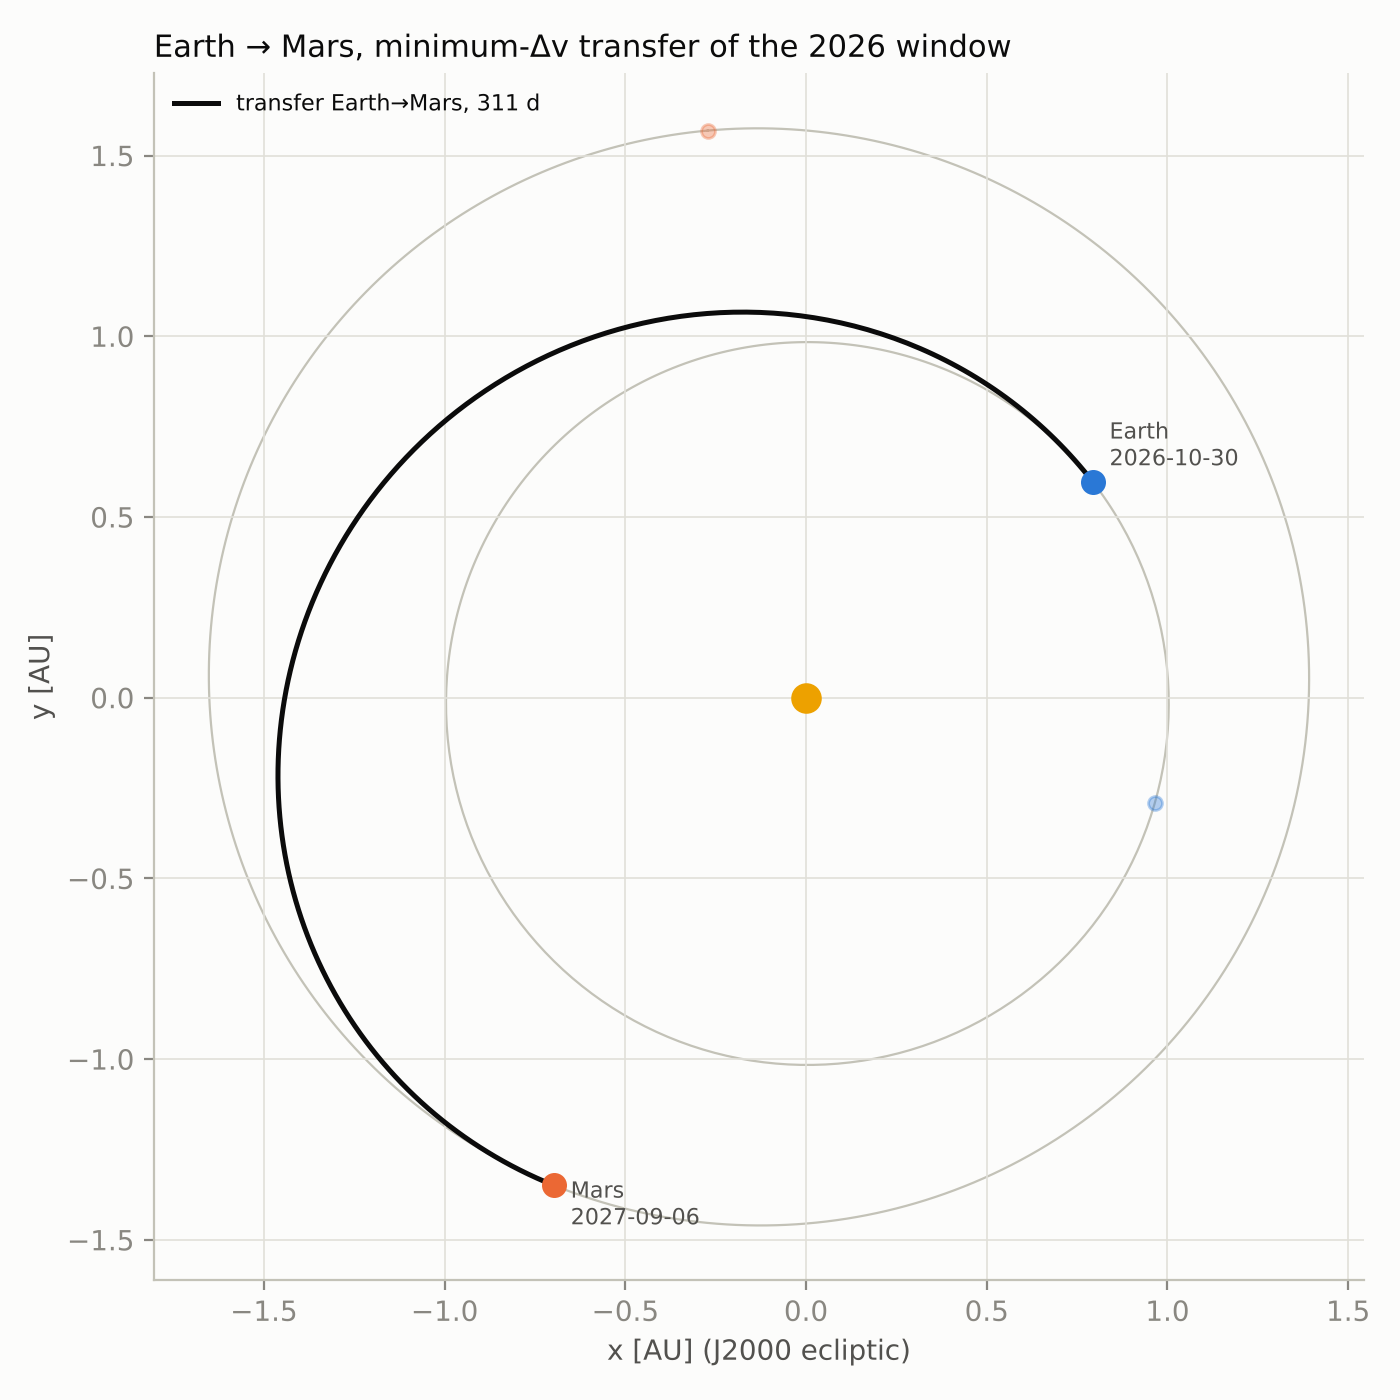
\includegraphics[width=\linewidth]{transfer_earth_mars_2026}\end{minipage}
\caption{Earth$\to$Mars 2026/27. Left: total $\dv$ (300-km parking orbit to 400-km Mars orbit) with $C_3$ contours and time-of-flight lines. Right: the minimum-$\dv$ transfer in plan view (type II, $\SI{\PkOptAngle}{\degree}$ of heliocentric travel).}
\label{fig:porkchop}
\end{figure}

\begin{worked}{The window opening now}
Grid: departures 2026-09-01 to 2027-02-15, flights 120--450 days. Minimum total $\dv$:
depart \PkOptDep, \SI{\PkOptTOF}{days}, $C_3=\SI{\PkOptCthree}{km^2/s^2}$,
$\vinf^{arr}=\SI{\PkOptvinfarr}{km/s}$, total \SI{\PkOptdv}{km/s} (type II). Minimum $C_3$:
\SI{\PkMinCthree}{km^2/s^2} on \PkMinCthreeDep\ with a \SI{\PkMinCthreeTOF}{day} flight.
Best type-I transfer: depart \PkTypeIDep, \SI{\PkTypeITOF}{days}, $C_3=\SI{\PkTypeICthree}{}$,
$\vinf^{arr}=\SI{\PkTypeIvinf}{km/s}$, total \SI{\PkTypeIdv}{km/s}---\SI{0.36}{km/s} more for
\SI{51}{days} less. Window within 10\% of the optimum: \PkWinOpen\ to \PkWinClose\ (\SI{\PkWinDays}{days}).
Check against reality: for Mars~2020 (launch 2020-07-30, entry 2021-02-18) the same machinery gives
$C_3=\SI{\MtwCthree}{km^2/s^2}$, a \SI{\Mtwdtheta}{\degree} type-I transfer and a heliocentric path
of \SI{\MtwPath}{Mkm} against the \SI{471}{Mkm} in NASA's press kit.
\end{worked}

\begin{codebox}
\code{lambert.py}: \code{lambert(r1, r2, tof, mu, prograde)} returning $\bv v_1$, $\bv v_2$, the
transfer angle and $a$. \code{porkchop.py}: \code{porkchop} (grids of $C_3$, $\vinf^{arr}$, $\dv$),
\code{Porkchop.optimum}, \code{Porkchop.window}, \code{next\_launch\_windows} (multi-year scan).
\code{plotting.plot\_porkchop}, \code{plot\_transfer}.
\end{codebox}

\begin{pitfall}
A porkchop plot answers ``what does this date pair cost'', not ``is this trajectory flyable'':
it ignores the declination constraint, the arrival geometry (lighting, landing site) and
navigation margins. It is the first filter, not the last.
\end{pitfall}

\subsection*{Exercises}
\begin{enumerate}[label=5.\arabic*,nosep]
\item Solve the type-I leg 2026-11-16 $\to$ 2027-08-03 and report $C_3$, $\vinf^{arr}$, transfer angle.
\item Why is time of flight monotonic in $z$ (\cref{fig:lambert}) but not in $a$? (Hint: the minimum-energy ellipse.)
\item Explain why the porkchop lobes are bounded on the left by an almost vertical wall for short flights.
\end{enumerate}

%==================================================================
\chapter{The Moon: a patched conic at small scale}\label{ch:moon}
%==================================================================

\section{Why the Moon is different}
The Moon's sphere of influence (\SI{\MoonSOI}{km}) is \SI{\MoonSOIfrac}{\percent} of the Earth--Moon
distance $D=\SI{\MoonD}{km}$, and the Moon moves at \SI{\MoonV}{km/s}---comparable to a
spacecraft's speed when it arrives. Neither ``SOI is a point'' nor ``target is stationary''
holds, so the patched conic must keep the geometry explicitly. It still works remarkably well.

\section{Level 1: Hohmann to the Moon}
Treat the Moon as a point at the apogee of a transfer ellipse from the parking orbit
($r_0=\SI{6563}{km}$ for 185~km): $a_t=\SI{\Lunat}{km}$, injection speed $v_0=\SI{\LunTLIv}{km/s}$
against circular \SI{\Lunvpark}{km/s}, so the trans-lunar injection (TLI) burn is
$\dv_{TLI}=\SI{\LunTLIdv}{km/s}$ with a flight of \SI{\LunTOFd}{days}. At apogee the spacecraft
moves at \SI{\Lunvapo}{km/s}, the Moon at \SI{\MoonV}{km/s}: the relative speed
$\vinf=\SI{\Lunvinf}{km/s}$ becomes the excess speed of a selenocentric hyperbola, and
\cref{eq:capture} gives lunar orbit insertion into a 100-km circular orbit:
$\dv_{LOI}=\SI{\LunLOIvhyp}{}-\SI{\LunLOIvc}{}=\SI{\LunLOI}{km/s}$. Total \SI{\Luntot}{km/s}.
These are the right magnitudes (Apollo flew \SI{3.05}{}--\SI{3.2}{km/s} TLI and \SI{0.9}{km/s} LOI).

\section{Level 2: the Bate--Mueller--White patched conic}
\Cref{fig:lunar} defines the geometry. Inputs: the injection state---radius $r_0$, speed $v_0$,
flight-path angle $\phi_0$ (angle of the velocity above the local horizontal)---and the arrival
angle $\lambda_1$, which places the point where the trajectory crosses the Moon's SOI.
\begin{enumerate}[nosep]
\item \textbf{Geocentric conservation.} $\En=v_0^2/2-\mu/r_0$ and $h=r_0v_0\cos\phi_0$ are
      constant on the geocentric leg.
\item \textbf{Arrival geometry.} The SOI point is at distance $r_1=\sqrt{D^2+r_{SOI}^2-2Dr_{SOI}\cos\lambda_1}$
      from Earth, at an angle $\gamma_1$ from the Earth--Moon line with $\sin\gamma_1=(r_{SOI}/r_1)\sin\lambda_1$.
\item \textbf{Arrival state.} $v_1=\sqrt{2(\En+\mu/r_1)}$ and $\cos\phi_1=h/(r_1v_1)$ from the two conserved quantities.
\item \textbf{Patch.} The selenocentric velocity is the vector difference
      $\bv v_2=\bv v_1-\bv v_{Moon}$, with $\bv v_{Moon}$ perpendicular to the Earth--Moon line.
      Its magnitude and direction relative to the Moon-centred radius vector give
      $\En_2=v_2^2/2-\mu_M/r_{SOI}$ and $h_2=|\bv\rho\times\bv v_2|$, hence
      $e_2=\sqrt{1+2\En_2h_2^2/\mu_M^2}$ and the perilune radius $r_p=h_2^2/[\mu_M(1+e_2)]$.
      The sign of $(\bv\rho\times\bv v_2)_z$ says whether the spacecraft passes the Moon
      prograde or retrograde.
\item \textbf{Time.} Kepler's equation on the geocentric ellipse from $r_0$ to $r_1$, plus the
      hyperbolic Kepler equation from $r_{SOI}$ to perilune (\SIrange{14}{18}{h}---not negligible).
      The Moon's lead angle at TLI follows from the two times and $\omega_{Moon}$.
\end{enumerate}
In practice one wants a given perilune altitude; the package scans $\lambda_1$ (for a chosen
$v_0$) or $v_0$ (for a chosen $\lambda_1$) and returns the solutions---usually one prograde and one
retrograde.

\begin{figure}[htb]\centering
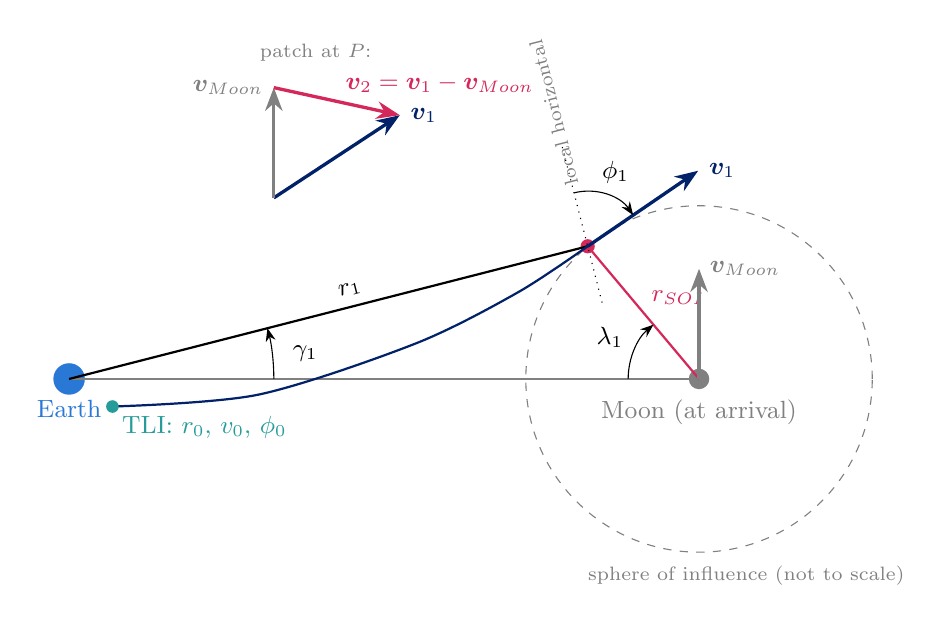
\begin{tikzpicture}[scale=1.0,>=Stealth]
  \def\D{8}\def\Rs{2.2}\def\lam{50}
  \fill[sfblue] (0,0) circle (0.2) node[below=4pt] {\small Earth};
  \fill[gray] (\D,0) circle (0.13) node[below=4pt] {\small Moon (at arrival)};
  \draw[dashed,gray] (\D,0) circle (\Rs); \node[gray,font=\scriptsize] at (\D+0.6,-\Rs-0.3) {sphere of influence (not to scale)};
  \draw[gray,thin] (0,0) -- (\D,0);
  \coordinate (P) at ({\D-\Rs*cos(\lam)},{\Rs*sin(\lam)});
  \fill[CUmagenta] (P) circle (0.09);
  \draw[thick] (0,0) -- (P) node[pos=0.55,above,sloped] {\small $r_1$};
  \draw[CUmagenta,thick] (\D,0) -- (P) node[midway,above right=-1pt] {\small $r_{SOI}$};
  \draw[->] (\D-0.9,0) arc (180:180-\lam:0.9); \node at ({\D-1.25*cos(\lam/2)},{1.25*sin(\lam/2)}) {\small $\lambda_1$};
  \draw[->] (2.6,0) arc (0:14.4:2.6); \node at (3.0,0.32) {\small $\gamma_1$};
  % Moon velocity
  \draw[->,very thick,gray] (\D,0) -- (\D,1.4) node[right] {\small $\bv v_{Moon}$};
  % local horizontal at P (perpendicular to r1) and v1 at phi1 above it
  \pgfmathsetmacro{\gam}{atan2(\Rs*sin(\lam),\D-\Rs*cos(\lam))}
  \draw[dotted] ($(P)+({1.3*cos(\gam+90)},{1.3*sin(\gam+90)})$) -- ($(P)+({-0.8*cos(\gam+90)},{-0.8*sin(\gam+90)})$);
  \node[font=\scriptsize,gray,rotate=\gam+90] at ($(P)+({1.75*cos(\gam+90)},{1.75*sin(\gam+90)})$) {local horizontal};
  \draw[->,very thick,CUblue] (P) -- ($(P)+({1.7*cos(\gam+90-70)},{1.7*sin(\gam+90-70)})$) node[right] {\small $\bv v_1$};
  \draw[->] ($(P)+({0.7*cos(\gam+90)},{0.7*sin(\gam+90)})$) arc (\gam+90:\gam+20:0.7);
  \node at ($(P)+({1.0*cos(\gam+55)},{1.0*sin(\gam+55)})$) {\small $\phi_1$};
  % geocentric transfer arc sketch
  \draw[CUblue,thick] plot[smooth] coordinates {(0.55,-0.35) (2.4,-0.2) (4.4,0.45) (5.7,1.1) (P)};
  \fill[CUteal] (0.55,-0.35) circle (0.08) node[below right] {\small TLI: $r_0,\,v_0,\,\phi_0$};
  % velocity triangle inset
  \begin{scope}[shift={(2.6,2.3)}]
    \node[font=\scriptsize,gray,anchor=west] at (-0.3,1.85) {patch at $P$:};
    \draw[->,very thick,CUblue] (0,0) -- (1.6,1.05) node[right] {\small $\bv v_1$};
    \draw[->,very thick,gray] (0,0) -- (0,1.4) node[left] {\small $\bv v_{Moon}$};
    \draw[->,very thick,CUmagenta] (0,1.4) -- (1.6,1.05) node[pos=0.5,above right=-1pt,font=\small] {$\bv v_2=\bv v_1-\bv v_{Moon}$};
  \end{scope}
\end{tikzpicture}
\caption{Bate--Mueller--White lunar patched conic. The arrival angle $\lambda_1$ fixes where the geocentric ellipse meets the Moon's sphere of influence; $r_1$ and $\gamma_1$ follow from the triangle Earth--Moon--$P$, the arrival speed and flight-path angle $\phi_1$ from energy and angular momentum, and subtracting the Moon's velocity (inset) gives the selenocentric hyperbola.}
\label{fig:lunar}
\end{figure}

\begin{worked}{Two transfers with $v_0=\SI{10.95}{km/s}$ from 185 km}
Geocentric ellipse: $a=\SI{\LunRa e3}{km}$, $e=\LunRe$; TLI $\dv=\SI{\LunRTLI}{km/s}$.
\emph{Retrograde solution} (Apollo-like): $\lambda_1=\SI{\LunRlam}{\degree}$, $r_1=\SI{\LunRrone e3}{km}$,
$v_1=\SI{\LunRvone}{km/s}$, $\phi_1=\SI{\LunRphione}{\degree}$, $\gamma_1=\SI{\LunRgammaone}{\degree}$;
$\vinf=\SI{\LunRvinf}{km/s}$, $e_2=\LunRetwo$, perilune 100~km, LOI \SI{\LunRLOI}{km/s};
\SI{\LunRtofgeo}{h} to the SOI $+$ \SI{\LunRtofsoi}{h} to perilune $=$ \SI{\LunRtoftot}{h}; Moon
lead angle at TLI \SI{\LunRlead}{\degree}.
\emph{Prograde solution}: $\lambda_1=\SI{\LunPlam}{\degree}$, $\vinf=\SI{\LunPvinf}{km/s}$, LOI \SI{\LunPLOI}{km/s},
\SI{\LunPtoftot}{h}.
Apollo~11's published TLI state (\SI{10.832}{km/s} at \SI{336}{km}, flight-path angle $\approx7^\circ$)
gives \SI{\ApTOF}{h} to perilune and LOI \SI{\ApLOI}{km/s}; the S-IVB cutoff row of the same
table (\SI{10.840}{km/s} at \SI{323}{km}) gives \SI{\ApTOFtwo}{h}. Apollo~11 took \SI{73.0}{h} and
burned \SI{0.891}{km/s}. Lunar time of flight moves about \SI{5}{h} per \SI{0.1}{km^2/s^2} of
injection energy, so the spread reflects the published altitude datum, not the method.
\end{worked}

\begin{codebox}
\code{lunar.py}: \code{lunar\_hohmann\_estimate}; \code{lunar\_patched\_conic(r0, v0, phi0, lambda1)};
\code{design\_lunar\_transfer(park\_alt, perilune\_alt, v0=.. | lambda1\_deg=..)};
\code{LunarPatchedConic.loi\_dv}, \code{.tof\_total}, \code{.direction}. \code{plotting.plot\_lunar\_transfer}.
\end{codebox}

\begin{pitfall}
Omitting the time from the SOI to perilune under-predicts lunar flight time by 15--20\%; it is the
first thing to check when a patched-conic lunar result disagrees with a flown mission.
\end{pitfall}

\subsection*{Exercises}
\begin{enumerate}[label=6.\arabic*,nosep]
\item Find the retrograde solution for $v_0=\SI{11.0}{km/s}$ from 185~km to a 100-km perilune: $\lambda_1$, total time, LOI.
\item Why does a faster transfer (larger $v_0$) cost more LOI even though TLI rises only slightly?
\end{enumerate}

%==================================================================
\chapter{Getting to orbit}\label{ch:launch}
%==================================================================
Everything so far started in a parking orbit. The launch itself is a trajectory problem (gravity
turn, drag, steering) treated in the Week-10 lecture and by the course's ascent-trajectory tool;
mission analysis only needs a defensible $\dv$:
\begin{keyresult}
\begin{equation}
  \dv_{launch}=\big|\bv v_{orbit}-\bv v_{site}\big|+\dv_{grav}+\dv_{drag}+\dv_{steer}.
\end{equation}
\end{keyresult}
The launch site already moves eastward with Earth's rotation,
$v_{site}=\omega_\oplus R\cos\phi_L$ ($\omega_\oplus=\SI{\LchOmega}{rad/s}$, \SI{\LchVeq}{km/s}
at the equator). To reach inclination $i$ from latitude $\phi_L$ the launch azimuth $Az$ (from
north) satisfies $\cos i=\cos\phi_L\sin Az$, which requires $i\ge\phi_L$: a site cannot reach an
inclination lower than its latitude without a plane change. The ideal $\dv$ is the vector
difference between the orbital velocity at that azimuth and the eastward site velocity; losses
are added as a band (gravity 1.0--1.5, drag 0.05--0.15, steering 0.1--0.4~km/s are typical for
medium launchers).

\begin{worked}{Kennedy Space Center ($\phi_L=28.5^\circ$) to 300 km}
Due east ($i=28.5^\circ$): $v_{orbit}=\SI{\LchVorb}{km/s}$, $v_{site}=\SI{\LchVsite}{km/s}$,
ideal $\dv=\SI{\LchIdeal}{km/s}$, with losses \SIrange{\LchLow}{\LchHigh}{km/s}.
To the ISS inclination ($51.6^\circ$, $Az=\SI{\LchISSaz}{\degree}$): credit \SI{\LchISScredit}{km/s},
ideal \SI{\LchISSideal}{km/s}. Polar: credit \SI{\LchPolarCredit}{km/s} (slightly negative---the
site velocity is now sideways), ideal \SI{\LchPolarIdeal}{km/s}. Kourou ($5.2^\circ$) due east
gains \SI{\LchKourouCredit}{km/s}.
\end{worked}

\begin{codebox}
\code{launch.py}: \code{launch\_to\_orbit(altitude, inclination\_deg, latitude\_deg, body, losses)},
\code{LossBand}, \code{dv\_to\_escape\_from\_orbit}.
\end{codebox}

\begin{pitfall}
The sign: $\dv=v_{orbit}+\text{losses}-v_{site}$. Earth's rotation \emph{helps} an eastward launch.
(The 2025 Week-9 slide had the signs reversed; the corrected estimate is \SIrange{8.9}{9.4}{km/s}
with the slide's 1.5--2.0~km/s loss band.)
\end{pitfall}

%==================================================================
\chapter{Aero-assist: trading heat shield for propellant}\label{ch:aero}
%==================================================================

\section{Aerocapture}
If the target has an atmosphere, one deep pass can remove the hyperbolic excess energy instead
of the capture burn. The spacecraft enters at
$v_{entry}=\sqrt{\vinf^2+2\mu/r_{atm}}$ (\SI{\AcEntry}{km/s} at Mars for $\vinf=\SI{\EMvinfarr}{km/s}$),
emerges on an ellipse whose periapsis is still in the atmosphere, and raises it with a small
apoapsis burn (\SI{\AcRaise}{km/s} here). The budget credit is the whole propulsive capture,
\SI{\AcSaved}{km/s} for a 400-km orbit---paid for with a heat shield, a guided entry and a narrow
corridor of acceptable entry angles. The tool charges only the $\dv$ side of that trade.

\section{Aerobraking}
Less demanding is to capture propulsively into a high ellipse (\SI{\AbCapHigh}{km/s} into
$110\times\SI{40000}{km}$ at Mars) and lower the apoapsis over hundreds of shallow passes through
the upper atmosphere. Each pass removes a little speed at periapsis. With an exponential
atmosphere $\rho=\rho_p\exp[-(r-r_p)/H]$, drag deceleration $\dd v/\dd t=-\rho v^2/(2\beta)$
($\beta=m/C_DA$ the ballistic coefficient) and the radius near periapsis expanded as
$r-r_p\approx\tfrac12\ddot r_pt^2$, the integral over a pass is Gaussian:
\begin{keyresult}
\begin{equation}
  \dv_{pass}=\frac{\rho_pV_p^2}{2\beta}\sqrt{\frac{2\pi H}{\ddot r_p}},\qquad
  \ddot r_p=\frac{V_p^2}{r_p}-\frac{\mu}{r_p^2}.
  \label{eq:aero}
\end{equation}
\end{keyresult}
$\ddot r_p$ is the radial acceleration at periapsis: the centripetal term of the curved path minus
gravity. Dropping gravity (a straight-line fly-through) gives the compact form
$\rho_pV_p\sqrt{2\pi Hr_p}/(2\beta)$ found on the lecture slide, which is low by the factor
$\sqrt{V_p^2/(V_p^2-\mu/r_p)}$---$\sqrt2$ for a near-parabolic pass, more for lower apoapses.
Direct integration of the equations of motion with drag confirms \cref{eq:aero} to 0.2\%
(\cref{fig:aero}). Pass after pass the apoapsis falls, periods shorten, and a final periapsis-raise
burn circularizes.

\begin{figure}[htb]\centering
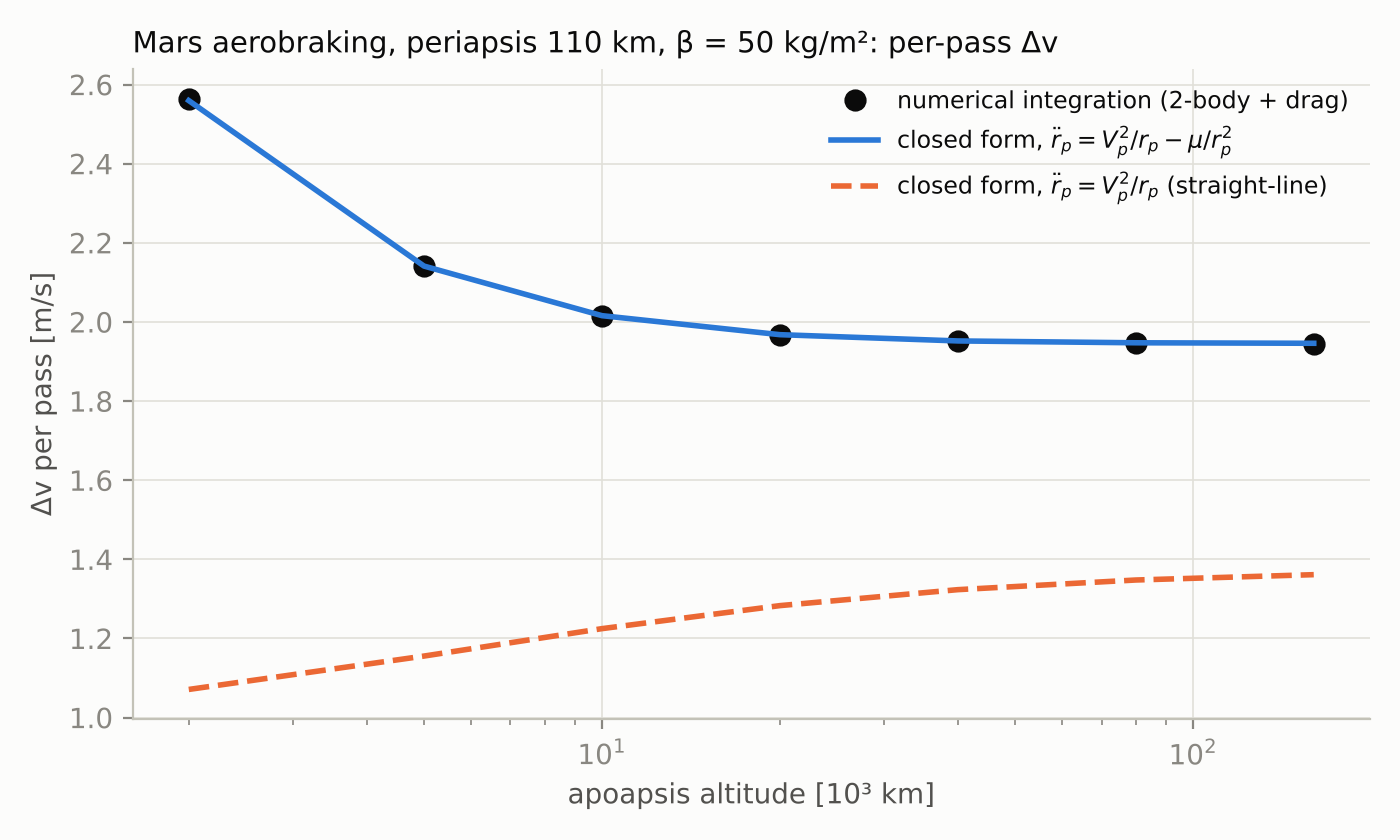
\includegraphics[width=0.7\textwidth]{aerobraking_pass_comparison}
\caption{Per-pass $\dv$ at Mars (periapsis 110 km, $\beta=\SI{50}{kg/m^2}$): integration versus the two closed forms.}
\label{fig:aero}
\end{figure}

\begin{worked}{Mars aerobraking campaign}
$\rho_p=\SI{\AbRho}{kg/m^3}$ at 110 km, $H=\SI{\AbH}{km}$, $V_p=\SI{\AbVp}{km/s}$,
$\ddot r_p=\SI{\AbRddot}{m/s^2}$, $\beta=\SI{50}{kg/m^2}$: first pass $\dv=\SI{\AbFirst}{m/s}$
(integration \SI{\AbNum}{}, gravity-aware \SI{\AbAna}{}, straight-line \SI{\AbStraight}{m/s}).
From $110\times\SI{40000}{km}$ to a circular 400-km orbit: \AbPasses\ passes over \SI{\AbDays}{days},
\SI{\AbDrag}{km/s} removed by drag, final raise \SI{\AbRaise}{km/s}. Propulsive total
$\SI{\AbCapHigh}{}+\SI{\AbRaise}{}$ versus direct capture \SI{\AbDirect}{km/s}: saving
\SI{\AbSaved}{km/s}. Halving the drag area (doubling $\beta$) doubles the passes and the
campaign time.
\end{worked}

\begin{codebox}
\code{aerobraking.py}: \code{aerocapture\_credit}, \code{aerobraking\_pass\_dv} (both closed forms),
\code{aerobraking\_pass\_dv\_numeric} (integrated check), \code{aerobraking\_campaign}.
Atmospheres: \code{Body.atmosphere} (exponential fits for the 90--150 km band).
\end{codebox}

%==================================================================
\chapter{From \texorpdfstring{$\dv$}{dv} to mass: the rocket equation and staging}\label{ch:staging}
%==================================================================
This is where the propulsion engineer takes over, so only the bridge is built here.

\section{The rocket equation in mission terms}
With $c=\gz\Isp$ ($\gz=\SI{\gzero}{m/s^2}$) the propellant fraction for a burn or a whole budget is
\begin{equation}
  \zeta=\frac{m_p}{m_0}=1-e^{-\dv/c},\qquad\text{and inversely}\qquad
  \Isp^{req}=\frac{\dv}{\gz\ln[1/(1-\zeta)]}.
\end{equation}
For a \SI{5.7}{km/s} budget: $\zeta=\ZetaThreeTwoZero$ at \SI{320}{s} (storable bipropellant),
$\ZetaFourFiveZero$ at \SI{450}{s} (hydrogen--oxygen), $\ZetaNineZeroZero$ at \SI{900}{s} (nuclear thermal),
$\ZetaThreeZeroZeroZero$ at \SI{3000}{s} (electric---if the mission can afford the time). A single stage to
orbit (\SI{9.3}{km/s}) with 90\% propellant fraction needs $\Isp=\SI{\IspSSTO}{s}$.

\section{Staging}
For stage $i$ (burning first for $i=1$) define the structural coefficient
$\sigma_i=m_{s,i}/(m_{s,i}+m_{p,i})$, the stage mass ratio $R_i=m_{0,i}/(m_{0,i}-m_{p,i})=e^{\dv_i/c_i}$
and the payload ratio $\pi_i=m_{0,i+1}/m_{0,i}$ (everything above stage $i$ is its payload).
Eliminating the stage mass,
\begin{keyresult}
\begin{equation}
  \pi_i=\frac{1-R_i\sigma_i}{R_i(1-\sigma_i)},\qquad
  \frac{m_0}{m_L}=\prod_i\frac{1}{\pi_i}=\prod_i\frac{R_i(1-\sigma_i)}{1-R_i\sigma_i},
\end{equation}
\end{keyresult}
which requires $R_i\sigma_i<1$: a stage with $\sigma_i=0.08$ cannot deliver more than
$c_i\ln(1/\sigma_i)$ even with zero payload. For a fixed total $\dv=\sum\dv_i$ the split that
minimizes $m_0$ follows from a Lagrange multiplier $\lambda$:
$R_i=(\lambda c_i-1)/(\lambda c_i\sigma_i)$ with $\sum c_i\ln R_i=\dv$---one scalar root; identical
stages give equal $\dv_i$. (The package names $\sigma_i$ \code{structural\_fraction} and reports
$\lambda_i=m_{0,i+1}/(m_{s,i}+m_{p,i})=\pi_i/(1-\pi_i)$ as \code{payload\_ratio}.)

\section{Budgets}
A \code{DeltaVBudget} is the hand-off object: an ordered list of legs (launch with its loss band,
injection, flybys, capture or aerocapture, landing, margin), each optionally tagged with the $\Isp$
of the stage that performs it. From it: the post-launch propulsive $\dv$, the propellant fraction at
a given $\Isp$, the required $\Isp$ at a given fraction, and the propellant per leg by working
backward from the final mass.

\begin{worked}{HW 1 chain: a Mars orbiter in the 2026 window}
Dates from the porkchop optimum (\HWdepart\ $\to$ \HWarrive). Legs: launch
\SI{\HWlaunchMid}{km/s} (band \SIrange{\LchLow}{\LchHigh}{}), injection \SI{\HWinj}{km/s},
capture \SI{\HWcap}{km/s}, 5\% margin \SI{\HWmargin}{km/s}: total \SI{\HWtotProp}{km/s}
(\SI{\HWtotAero}{km/s} with aerocapture). Post-launch propulsive $\dv$: \SI{\HWpostProp}{km/s}
vs.\ \SI{\HWpostAero}{km/s}. Required $\Isp$ at $\zeta=0.5/0.6/0.7$: \HWIspPropFive/\HWIspPropSix/\HWIspPropSeven~s
propulsive, \HWIspAeroFive/\HWIspAeroSix/\HWIspAeroSeven~s with aerocapture. A \SI{1000}{kg} final mass
with a 320-s engine (propulsive capture) needs \SI{\HWmpropMargin}{} (margin) $+$ \SI{\HWmpropCap}{}
(capture) $+$ \SI{\HWmpropInj}{kg} (injection) of propellant: \SI{\HWminj}{kg} injected onto
the escape hyperbola. A two-stage launcher ($\Isp$ 300/450~s, $\sigma$ 0.07/0.10) delivering that
mass through \SI{\HWdvLauncher}{km/s} (launch $+$ injection): optimal split \SI{\HWdvB}{}/\SI{\HWdvU}{km/s},
stage masses \SI{\HWmB}{}/\SI{\HWmU}{t}, gross \SI{\HWmZero}{t} (payload fraction \SI{\HWpf}{\percent});
an equal split would weigh \SI{\HWmZeroeq}{t}.
\end{worked}

\begin{codebox}
\code{staging.py}: \code{tsiolkovsky\_dv}, \code{propellant\_fraction\_for\_dv}, \code{required\_isp},
\code{design\_vehicle} (optimal split), \code{size\_vehicle}, \code{size\_burn\_sequence}.
\code{budget.py}: \code{DeltaVBudget} (\code{table}, \code{size\_propellant}, \code{required\_isp}),
\code{interplanetary\_budget}, \code{lunar\_budget}.
\end{codebox}

%==================================================================
\chapter{Putting it together}\label{ch:walkthrough}
%==================================================================
The chain below is what HW~1 asks for and what the project model begins with; each line is one
call into the package.

\begin{lstlisting}
from modern_aerospace_propulsion.mission_analysis import *

# 1. textbook orientation (Ch. 2-3): circular coplanar Hohmann
print(hohmann_interplanetary("Earth", "Mars", park_alt=300, capture_peri_alt=400).summary())

# 2. the real window (Ch. 4-5): porkchop over dated Lambert solutions
pc = porkchop("Earth", "Mars", "2026-09-01", "2027-02-15", 120, 450,
              park_alt=300, capture_peri_alt=400)
opt = pc.optimum("dv_total")               # depart, arrive, C3, v_inf, dv

# 3. the budget (Ch. 7-9): launch band + injection + capture (or aerocapture) + margin
budget, mission = interplanetary_budget("Earth", "Mars", opt["depart"], opt["arrive"],
                                        park_alt=300, launch_lat_deg=28.5,
                                        capture_peri_alt=400, aerocapture=False)
print(budget.table())

# 4. propellant and staging (Ch. 9)
rows = budget.size_propellant(final_mass=1000.0, default_isp=320.0)
m_injected = rows[0]["m_before"]
launcher = design_vehicle(budget.legs[0].dv + budget.legs[1].dv, m_injected,
                          isps=[300, 450], sigmas=[0.07, 0.10])
print(launcher.table())

# 5. levers (Ch. 3, 8): aerocapture, elliptical capture, gravity assist
print(aerocapture_credit("Mars", mission.capture.vinf, 400).summary())
print(capture_dv("Mars", mission.capture.vinf, 400, 40000).summary())
\end{lstlisting}

Read the output against this tutorial: the Hohmann numbers of \cref{tab:planets} bound the dated
ones; the porkchop optimum sits on the type-II lobe; the capture burn is \cref{eq:capture}; the
budget's propellant fraction is the rocket equation; and the launcher's optimal split is the
Lagrange result of \cref{ch:staging}. When a number surprises you, the chapter that owns it is
where to look.

\paragraph{What this model does not know.} Patched conics ignore third-body gravity during each
leg; burns are impulsive; the ephemeris is good to arcminutes; the Moon's orbit is taken
circular; aero-assist is charged only its $\dv$; launch losses are a band, not a trajectory.
The companion technical report quantifies each of these and names the remedy. For sizing a
propulsion system they are the right approximations; for flying, they are the first guess.

%==================================================================
\appendix
\chapter{Symbols}\label{app:symbols}
\begin{center}\small
\begin{tabular}{lp{0.78\textwidth}}\toprule
$\mu$ & gravitational parameter $GM$ [\si{km^3/s^2}] (only meaning) \\
$\En$ & specific mechanical energy $v^2/2-\mu/r=-\mu/(2a)$ \\
$\bv h$, $h$ & specific angular momentum $\bv r\times\bv v$ \\
$a$, $e$, $p$ & semi-major axis, eccentricity, semi-latus rectum $h^2/\mu$ \\
$r_p$, $r_a$ & periapsis, apoapsis radius \\
$\nu$, $E$, $M$, $F$ & true, eccentric, mean, hyperbolic anomaly \\
$n$, $T$ & mean motion $\sqrt{\mu/a^3}$, period \\
$i$, $\Omega$, $\omega$ & inclination, right ascension of the ascending node, argument of periapsis \\
$\Delta\theta$ & transfer angle between $\bv r_1$ and $\bv r_2$ \\
$f$, $g$ & Lagrange coefficients; $z$, $\chi$ universal variable and anomaly \\
$v_c$, $v_{esc}$ & circular and escape speed at a radius \\
$v_{t,p}$, $v_{t,a}$, $a_t$, $t_H$ & Hohmann transfer periapsis/apoapsis speeds, semi-major axis, flight time \\
$\vinf$, $C_3=\vinf^2$ & hyperbolic excess speed (relative to the planet), launch energy \\
$\delta$, $\beta$, $\Delta$ & flyby turning angle; periapsis-to-asymptote angle; aiming radius \\
$r_{SOI}$ & sphere-of-influence radius $a(m/M)^{2/5}$ \\
$\lambda_1$, $\gamma_1$, $\phi$ & lunar arrival angle; angle at Earth; flight-path angle (above local horizontal) \\
$\phi_L$, $Az$ & launch-site latitude, launch azimuth from north \\
$\beta$ (\cref{ch:aero}) & ballistic coefficient $m/(C_DA)$ [\si{kg/m^2}]; $H$, $\rho_p$ scale height and periapsis density \\
$\zeta$, $\sigma_i$, $\pi_i$, $R_i$ & propellant fraction $m_p/m_0$; structural coefficient $m_s/(m_s+m_p)$; payload ratio $m_{0,i+1}/m_{0,i}$; stage mass ratio $e^{\dv_i/c_i}$ \\
$c$, $\Isp$, $\gz$ & effective exhaust velocity $\gz\Isp$, specific impulse, \SI{9.80665}{m/s^2} \\\bottomrule
\end{tabular}
\end{center}

\chapter{Answers to exercises}\label{app:answers}
\begin{description}[style=nextline,leftmargin=0pt,itemsep=2pt]
\item[1.1] $v_c=\SI{\ExMarsVc}{km/s}$, $T=\SI{\ExMarsTmin}{min}$, $v_{esc}=\SI{\ExMarsVesc}{km/s}$.
\item[1.2] Perigee speed \SI{\EMvpark}{}$+3.5=\SI{11.23}{km/s}>v_{esc}=\SI{\ObvescLEO}{km/s}$: unbound. $\vinf=\sqrt{v^2-2\mu/r}=\SI{\ExVinfFromBurn}{km/s}$, $C_3=\SI{\ExCthreeFromBurn}{km^2/s^2}$.
\item[1.3] Half the period, \SI{\GTOhalfperiodmin}{min}: Kepler's equation is odd about $E=\pi$, so $M=\pi$ exactly at apoapsis for any $e$.
\item[2.1] $\dv_1=\SI{\ExLunHohdvone}{km/s}$, $\dv_2=\SI{\ExLunHohdvtwo}{km/s}$ ($v_{t,a}=\SI{\ExLunHohvta}{}$ vs.\ $v_c=\SI{\ExLunHohvcTwo}{km/s}$), $t_H=\SI{\ExLunHohtofd}{days}$. $\dv_1$ is the TLI of \cref{ch:moon} (\SI{\LunTLIdv}{km/s} from 185~km); $\dv_2$ is what the Moon's own gravity makes unnecessary---the Moon ``circularizes'' the spacecraft for the price of LOI.
\item[2.2] $\dv_2=v_{c,2}-v_{t,a}$; both terms fall with $r_2$, but $v_{t,a}\to0$ faster than $v_{c,2}\propto r_2^{-1/2}$ for small ratios and then both vanish; the difference peaks near $r_2/r_1\approx5.9$.
\item[2.3] Separately: \SI{\HohLEOGEOtot}{}$+$\SI{\PCatGEO}{}$=\SI{5.41}{km/s}$ (plane change at GEO) or $+\SI{\PCatLEO}{}$ at LEO; combined optimum \SI{\HohPCtot}{km/s}, with almost all of the angle taken at the slow apogee burn.
\item[3.1] $\vinf=\SI{\ExJupvinf}{km/s}$; circular 1000~km: hyperbolic speed \SI{\ExJupVhyp}{} vs.\ circular \SI{\ExJupVc}{km/s}, $\dv=\SI{\ExJupCapCirc}{km/s}$ (hopeless); ellipse to \SI{2e6}{km}: \SI{\ExJupCapEll}{km/s}. Circular optimum at an altitude of \SI{\ExJupOptAlt e3}{km}.
\item[3.2] $e=\ExVenE$, $\delta=\SI{\ExVenTurn}{\degree}$, $|\dv_{helio}|=\SI{\ExVenDv}{km/s}$.
\item[3.3] In the planet frame the encounter is a hyperbola with constant energy, so $|\bv\vinf|$ in equals out; the Sun-frame velocity adds the planet's velocity to a rotated $\bv\vinf$, and the magnitude of a sum depends on the angle between the vectors.
\item[5.1] $C_3=\SI{\ExLegCthree}{km^2/s^2}$, $\vinf^{arr}=\SI{\ExLegvinf}{km/s}$, transfer angle \SI{\ExLegAngle}{\degree} (type I), \SI{\ExLegTOF}{days}.
\item[5.2] For a given geometry two ellipses of the same $a>a_{min}$ connect the points (short and long arc), so $\Delta t(a)$ is double-valued; $z$ parametrizes the arc itself and is single-valued.
\item[5.3] Short flights need hyperbolic transfers whose $\vinf$---and hence $C_3$ and $\dv$---grow without bound as $\Delta t\to0$; the contours bunch into a wall.
\item[6.1] $\lambda_1=\SI{\ExLunLam}{\degree}$, \SI{\ExLunTOF}{h} to perilune, TLI \SI{\ExLunTLI}{km/s}, LOI \SI{\ExLunLOI}{km/s}.
\item[6.2] A faster transfer arrives at the Moon with a larger geocentric speed, hence a larger $\vinf$ relative to the Moon; LOI grows with $\vinf$ (\cref{eq:capture}) while TLI grows only with $v_0$ at perigee, where the Oberth effect makes energy cheap.
\end{description}

\chapter{Further reading}
Bate, Mueller \& White, \emph{Fundamentals of Astrodynamics} (Dover): the clearest first book,
and the source of the lunar method of \cref{ch:moon}. Curtis, \emph{Orbital Mechanics for
Engineering Students}: algorithms with worked numbers, the reference for the universal-variable
and Lambert code. Vallado, \emph{Fundamentals of Astrodynamics and Applications}: the
practitioner's handbook. Sutton \& Biblarz, \emph{Rocket Propulsion Elements}, Ch.~4: the
propulsion side of the same story. The companion technical report in \code{docs/report/} documents
the implementation, validation and limitations of the package in full.

\end{document}
